\documentclass{article}

\usepackage[UKenglish]{babel}
\usepackage[utf8]{inputenc}
\usepackage[a4paper, margin=20mm]{geometry}
\usepackage{textcomp} % makes the "not defining \perthousand"/"\micro" errors go away by including this first
\usepackage{amsmath}
\usepackage{amssymb}
\usepackage{amsthm}
\usepackage{amsfonts}
\usepackage{wrapfig}
\usepackage{physics}
\usepackage{bm}
\DeclareDocumentCommand\mathbf{m}{\bm{\mathrm{#1}}} % make bold work for greek symbols
\DeclareDocumentCommand\vnabla{}{\nabla} % use non-bold nabla for \grad, \curl etc. Enabled to unify laplacian symbol between vector and scalar forms
\DeclareDocumentCommand\dotproduct{}{\cdot} % use non-bold dot for scalar product to unify notation
\DeclareDocumentCommand\crossproduct{}{\times} % use non-bold dot for scalar product to unify notation
\usepackage{gensymb}
\usepackage{enumerate}
\usepackage{mathtools}
\usepackage{centernot}
\usepackage{relsize}
\usepackage{mathrsfs}
\usepackage{siunitx}
\usepackage{pgfplots}
\pgfplotsset{width=10cm,compat=1.9}
\usepgfplotslibrary{external}
\tikzexternalize[prefix=tikz/]
\usepackage[pdfa]{hyperref}
\hypersetup{
	colorlinks=true,
	linktoc=all,
	linkcolor=black,
}

\numberwithin{equation}{section} % make equations be numbered 1.1 not 1

\newcommand{\tableofcontentsnewpage}{\tableofcontents\newpage}

% create the theorem environments
\theoremstyle{definition}
\newtheorem*{definition}{Definition}

\newtheorem*{claim}{Claim}
\newtheorem*{theorem}{Theorem}
\newtheorem*{proposition}{Proposition}
\newtheorem*{lemma}{Lemma}
\newtheorem*{corollary}{Corollary}

\theoremstyle{remark}
\newtheorem*{note}{Note}
\newtheorem*{remark}{Remark}

\newcommand{\ddempty}{\mathrm{d}}
\newcommand{\dn}[2]{\mathrm{d}^#1#2}
\newcommand{\st}{\text{ s.t. }}
\newcommand{\contradiction}{\(\#\)}
\newcommand{\genset}[1]{\langle{} #1 \rangle}
\newcommand{\nhat}{\vu{n}}
\newcommand{\rdot}{\dot{\vb{r}}}
\newcommand{\rddot}{\ddot{\vb{r}}}
\newcommand{\transpose}{\intercal}
\newcommand{\acts}{\curvearrowright}
\newcommand{\adjugate}[1]{\widetilde{#1}}
\newcommand{\mathhuge}[1]{\mathlarger{\mathlarger{\mathlarger{#1}}}}
\newcommand{\stcomp}[1]{{#1}^c} % consider \complement? Personally I think this looks better, and it's what Wikipedia uses
\newcommand{\prob}[1]{\mathbb{P}\left({#1}\right)}
\newcommand{\psub}[2]{\mathbb{P}_{#1}\left({#2}\right)}
\newcommand{\psubx}[1]{\psub{x}{#1}}
\newcommand{\expect}[1]{\mathbb{E}\left[{#1}\right]}
\newcommand{\esub}[2]{\mathbb{E}_{#1}\left[{#2}\right]}
\newcommand{\esubx}[1]{\esub{x}{#1}}
\newcommand{\Var}[1]{\Varop\left({#1}\right)}
\newcommand{\Cov}[1]{\Covop\left({#1}\right)}
\newcommand{\Corr}[1]{\Corrop\left({#1}\right)}
\newcommand{\convdist}{\xrightarrow{d}}
\newcommand{\convprob}{\xrightarrow{\mathbb{P}}}

\DeclareMathOperator{\vecspan}{span}
\DeclareMathOperator{\HCF}{HCF}
\DeclareMathOperator{\LCM}{LCM}
\DeclareMathOperator{\ord}{ord}
\DeclareMathOperator{\Sym}{Sym}
\DeclareMathOperator{\nullity}{null}
\DeclareMathOperator{\Orb}{Orb}
\DeclareMathOperator{\Stab}{Stab}
\DeclareMathOperator{\ccl}{ccl}
\DeclareMathOperator{\Varop}{Var}
\DeclareMathOperator{\Covop}{Cov}
\DeclareMathOperator{\Corrop}{Corr}

\DeclarePairedDelimiter\ceil{\lceil}{\rceil}
\DeclarePairedDelimiter\floor{\lfloor}{\rfloor}

% for arrows in the middle of the line
\usetikzlibrary{decorations.markings}
\tikzset{->-/.style={decoration={
		markings,
		mark=at position #1 with {\arrow{>}}},postaction={decorate}}}


\title{Dynamics and Relativity}
\author{Cambridge University Mathematical Tripos: Part IA}

\begin{document}
\maketitle

\tableofcontentsnewpage{}

\section{Basic definitions and Newton's laws}
\subsection{Basic concepts}
\begin{definition}
	A particle is an object which has negligible size.
	It therefore does not have an alignment or rotation.
	It has a finite mass \(m > 0\), and perhaps an electric charge \(q\) (which may be positive or negative).
	The position of the particle is described by a position vector \(\vb r(t)\) or \(\vb x(t)\), with respect to an origin \(O\).
\end{definition}
\begin{definition}
	The Cartesian components of this vector \(\vb r(t)\) are given by \((x, y, z)\), where \(\vb r = x \hat{\textbf{\i}} + y \hat{\textbf{\j}} + z \hat{\textbf{k}}\), with \(\hat{\textbf{\i}}, \hat{\textbf{\j}}, \hat{\textbf{k}}\) orthonormal.
	The choice of coordinate axes defines a frame of reference \(S\).
\end{definition}
\begin{definition}
	The velocity of a particle is \(\vb u(t) = \dot{\vb r} = \frac{\dd}{\dd{t}}\vb r(t)\).
	The velocity is tangential to the path, or \textit{trajectory}, of the particle.
\end{definition}
\begin{definition}
	The momentum of a particle is \(\vb p = m \vb u\).
\end{definition}
\begin{definition}
	The acceleration of a particle is \(\vb a = \dot{\vb u} = \ddot{\vb r}\).
\end{definition}
\begin{note}
	The time derivative of \(\vb u(t)\), for example, is defined using the limit definition:
	\[
		\dot{\vb u}(t) = \lim_{h \to 0} \frac{\vb u(t + h) - \vb u(t)}{h}
	\]
	with \(\vb u \to \vb u_0\) if and only if \(\abs{\vb u - \vb u_0} \to 0\).
	With Cartesian basis vectors, we can evaluate derivatives componentwise, bringing the differential operator inside each vector component.
\end{note}
The derivatives of scalar and vector functions interoperate as expected.
Suppose we have a scalar function \(f(t)\) and vector functions \(\vb g(t), \vb h(t)\), then for example we have
\[
	\frac{\dd}{\dd{t}}(f \vb g) = \frac{\dd{f}}{\dd{t}} \vb g + f \frac{\dd \vb g}{\dd{t}}
\]
\[
	\frac{\dd}{\dd{t}}(\vb g \cdot \vb h) = \frac{\dd \vb g}{\dd{t}}\cdot \vb h + \vb g \cdot \frac{\dd \vb h}{\dd{t}}
\]
\[
	\frac{\dd}{\dd{t}}(\vb g \times \vb h) = \frac{\dd \vb g}{\dd{t}}\times \vb h + \vb g \times \frac{\dd \vb h}{\dd{t}}
\]
Take note of the ordering of the terms involving \(\vb g\) and \(\vb h\) when using the vector product.

\subsection{Newton's laws of motion}
\begin{enumerate}
	\item (Galileo's Law of Inertia) There exist inertial frames of reference in which a particle remains at rest or moves in a straight line at constant speed (i.e.\ at constant velocity), unless it is acted on by a force.
	\item In an inertial frame of reference, the rate of change of momentum of a particle is equal to the force acting on it.
	\item To every action, there is an equal and opposite reaction.
	      The forces exerted between two particles are equal in magnitude and opposite in direction.
\end{enumerate}
Note that the second law is a statement about vectors.
All of these statements that we have made about particles can also be extended to finite bodies, composed of many particles.

\subsection{Boosts}
In an inertial frame, the acceleration of a particle is zero if the force acting on the particle is zero.
\[
	\ddot{\vb r} = \vb 0 \iff \vb F = \vb 0
\]
There is no unique inertial frame of reference.
If \(S\) is an inertial frame, then any other frame \(S'\) moving at constant velocity relative to \(S\) is also an inertial frame.
For example, suppose that \(S'\) is moving at speed \(v\) in the \(x\) direction.
Then here
\[
	x'=x-vt;\quad y'=y;\quad z'=z;\quad t'=t
\]
and we can generalise this to \(S'\) moving in an arbitrary direction relative to \(S\), i.e.
\[
	\vb r' = \vb r - \vb v t
\]
where \(\vb v\) is the velocity of \(S'\) relative to \(S\).
This type of transformation is known as a `boost'.
For a particle with position vector \(\vb r(t)\) in \(S\) (and position vector \(\vb r'(t)\) in \(S'\)), we can compute the velocity \(\vb u = \dot{\vb r}\) and acceleration \(\vb a = \ddot{\vb r}\) as follows:
\[
	\vb u' = \vb u - \vb v;\quad \vb a' = \vb a
\]
This can be seen by taking the derivative of the `boost' formula.

\subsection{Galilean transformations}
A general Galilean Transformation is any transformation that preserves inertial frames.
They are combinations of:
\begin{itemize}
	\item boosts \(\vb r' = \vb r - \vb vt\) where \(\vb v\) is constant,
	\item translations of space (moving the origin) \(\vb r' = \vb r - \vb r_0\) where \(r_0\) is constant,
	\item translations of time \(t' = t - t_0\) where \(t_0\) is constant,
	\item rotations and reflections in space \(\vb r' = R \vb r\) where \(R\) is a constant orthogonal matrix.
\end{itemize}
This set generates the Galilean group.
For any Galilean transformation we have
\[
	\ddot{\vb r} = \vb 0 \iff \ddot{(\vb r')} = \vb 0
\]

The principle of Galilean relativity is that the laws of Newtonian physics are the same in all inertial frames.
In other words, the laws of physics are always the same:
\begin{itemize}
	\item at any point in space
	\item at any point in time
	\item in any direction
	\item at any constant velocity
\end{itemize}
Any set of equations which describe Newtonian physics must preserve this Galilean invariant.
This shows that measurement of velocity cannot be absolute, it must be relative to a specific inertial frame of reference --- but conversely, measurement of acceleration \textit{is} absolute.

\subsection{Newton's second law}
For any particle subject to a force \(\vb F\), the momentum \(\vb p\) of the particle satisfies
\[
	\frac{\dd \vb p}{\dd{t}} = \vb F
\]
where \(\vb p = m \vb u\).
For this part of the course, let us assume that \(m\) is constant.
Then \(\vb F = \dot{\vb p} = m \vb a\).
We can interpret this value \(m\) as a measure of `reluctance to accelerate', i.e.\ its inertia.
If \(\vb F\) is specified as a function of \(\vb r, \dot{\vb r}, t\), then we have a second order differential equation for \(\vb r\).
In order to solve this equation, we must provide two initial conditions, such as \(\vb r_0\) and \(\dot{\vb r}_0\) at some initial time \(t_0\).
The trajectory of the particle is then determined for all future and past times.

\subsection{Gravitational force}
Consider two particles, one at \(\vb r_1\) and one at \(\vb r_2\).
Newton's law of gravitation states that the gravitational force on \(\vb r_1\) is given by
\[
	\vb F_1 = \frac{- G m_1 m_2 (\vb r_1 - \vb r_2)}{\abs{\vb r_1 - \vb r_2}^3}
\]
where \(G\) is the gravitational constant, and \(\vb F_2\) is given by \(-\vb F_1\).
Note that:
\begin{itemize}
	\item This is known as an inverse square law, since the magnitude of the output is proportional to the inverse of the square of the distance between the particles.
	\item This is an attractive force, since it is in the direction \(\vb r_2 - \vb r_1\).
	\item This obeys Newton's Third Law, since \(\vb F_2 = - \vb F_1\).
	\item By inspection, \(G\) must have dimension \(L^3 \cdot M^{-1} \cdot T^{-2}\), i.e.\ length cubed over mass over time squared.
\end{itemize}

\subsection{Electromagnetic force}
Consider a particle with electric charce \(q\), in the presence of an electric field \(\vb E(\vb r, t)\) and a magnetic field \(\vb B(\vb r, t)\).
The Lorentz force law states that
\[
	\vb F(\vb r, \dot{\vb r}, t) = q\left( \vb E + \dot{\vb r} \times \vb B \right)
\]
As an example, let \(\vb E = \vb 0\) everywhere, and let \(\vb B\) be a constant vector.
Then
\[
	m \ddot{\vb r} = q \dot{\vb r} \times \vb B
\]
We can solve this differential equation for \(\vb r\).
Let us choose axes such that \(\vb B = B \vu{z}\), i.e.\ \(\vb B\) is in the \(z\) direction.
Evaluating the cross product, \(m \ddot{z} = 0\), so \(z = z_0 + ut\) where \(z_0\) and \(u\) are constants.
Further,
\[
	m \ddot x = qB\dot y;\quad m \ddot y = -qB\dot x
\]
For convenience, let us define \(\omega = qB/m\), and then
\[
	x = x_0 - \alpha \cos(\omega(t - t_0));\quad x = y_0 + \alpha \sin(\omega(t - t_0))
\]
This describes circles in the \(x\)--\(y\) plane, and constant velocity motion in the \(z\) direction.
This results in a helix in the direction of the magnetic field, clockwise when viewed from the direction of \(\vb B\).

\section{Dimensional analysis}
\subsection{Choice of units}
Many problems in dynamics involve three basic dimensional quantities: length, mass and time.
These are commonly referred to using the symbols \(L\), \(M\) and \(T\), to be generic over the choice of unit system.
The dimensions of some quantity \(x\) can therefore be expressed in terms of powers of \(L\), \(M\), \(T\).
So the dimension of density is \(M \cdot L^{-3}\).
The dimension of force is \(M \cdot L \cdot T^{-2}\).

Only `power law' functions of these quantities are allowed; we are not allowed to exponentiate a dimensional quantity, for example.
This is because \(e^L = 1 + L + \frac{1}{2}L^2 + \dots\) would be comparing a dimensionless constant 1 with some length, and some area, and so forth.
This comparison does not make any sense.

We can choose a unit system that is convenient, for example SI units.
It defines the metre for \(L\), the kilogram for \(M\) and the second for \(T\).
So many other physical quantities can be formed from these.
For example, the SI unit for the gravitational constant is \si{\metre\cubed\per\kilogram\per\second\squared}.
In this unit system, we can say \(G = \SI{6.67e-11}{\metre\cubed\per\kilogram\per\second\squared}\).

As a general principle, dynamical and physical equations must work for any consistent choice of units.
If, however, we used SI units for length, mass and time, but the imperial unit pound-force as the unit for force, the equations would be inconsistent.

\subsection{Scaling and dimensional independence}
Suppose that a dimensional quantity \(Y\) depends on a set of dimensional quantities \(X_1, \dots, X_n\), so the dimension of \(Y\) is \(L^a M^b T^c\) and the dimension of the \(X_i\) are \(L^{a_i} M^{b_i} T^{c_i}\).

If \(n \leq 3\), then \(Y = C \cdot X_1^{p_1}X_2^{p_2}X_3^{p_3}\), and \(p_1, p_2, p_3\) can be found by balancing the dimensions.
Hence \(a = a_1p_1 + a_2p_2 + a_3p_3\) and so forth for \(b\) and \(c\).
This yields a unique solution for \(p_1, p_2, p_3\) if these three equations are linearly independent, i.e.\ if the dimensions of \(X_1, X_2, X_3\) are independent.

If \(n > 3\), then this property of dimensional independence does not hold; it is always possible to express one of the four (or more) dimensions in terms of the other three.
So let us choose \(X_1, X_2, X_3\) to be dimensionally independent, and then we can incorporate \(X_4, X_5\) and so on as dimensionless quantities:
\[
	\lambda_1 = \frac{X_4}{X_1^{q_{11}}X_2^{q_{12}}X_3^{q_{13}}};\quad \lambda_2 = \frac{X_5}{X_1^{q_{21}}X_2^{q_{22}}X_3^{q_{23}}} \cdots
\]
where the powers \(q_{ij}\) have been chosen such that the \(\lambda\) are dimensionless.
Then
\[
	Y = X_1^{p_1}X_2^{p_2}X_3^{p_3} \cdot C(\lambda_1, \lambda_2, \dots, \lambda_{n-3})
\]
This is known as Bridgman's Theorem.

\begin{example}
	As an example, let us consider a simple pendulum with a string of length \(\ell\), released from rest, when the horizontal distance from the end of the pendulum to the rest position is \(d\).
	How does the period \(P\) of the pendulum depend on the four dimensional quantities \(m, \ell, d, g\)?

	We know that the dimension of the period is \(T\), time.
	The dimension of \(m\) is \(M\), the dimension of \(g\) is \(L \cdot T^{-2}\), and the dimensions of \(\ell\) and \(d\) are both \(L\).
	We will form one dimensionless group, since \(n=4\) in this case.
	A simple way of doing so is letting \(\lambda = d/\ell\).
	So \(P = m^{p_1} \ell^{p_2} g^{p_3} \cdot f(d/\ell)\).
	Comparing units, we have \(T = M^{p_1} L^{p_2} (L \cdot T^{-2})^{p_3}\).
	Solving, we get \(p_1 = 0, p_2 = \frac{1}{2}, p_3 = \frac{-1}{2}\).
	Applying Bridgman's Theorem, we have \(P = \sqrt{\ell / g} \cdot f(d/\ell)\).
	This does not completely specify the formula, but it does provide useful insights.
	For example, doubling both \(d\) and \(\ell\), \(P \mapsto \sqrt{2} P\), since \(d/\ell\) does not change.
\end{example}

\begin{example}
	Taylor used publicly available data on the fireball's growth over time in order to estimate the energy released in the first atomic explosion.
	Let \(R(t)\) be the radius of the fireball as a function of time, which has dimension \(L\).
	The time \(t\) has dimension \(T\).
	The density of air \(\rho\) has dimension \(M \cdot L^{-3}\).
	The energy of the explosion is \(E\) which has dimension \(M \cdot L^2 \cdot T^{-2}\).
	Then, \(R = C \cdot t^\alpha \rho^\beta E^\gamma\).
	By balancing dimensions, we have \(\alpha = \frac{2}{5}, \beta = \frac{-1}{5}, \gamma = \frac{1}{5}\).
	Then, \(R(t) = C \cdot t^{\frac{2}{5}} \rho^{\frac{-1}{5}} \gamma^{\frac{1}{5}}\).

	Taylor then verified this \(\frac{2}{5}\) power law, and estimated the value of \(E\) as \(\frac{\rho R^5}{C^5 t^2}\).
	It was observed that \(\frac{R^5}{t^2} \sim \SI{6.7e13}{\metre\tothe{5}\per\second}\), and \(\rho\sim\SI{1.25}{\kilogram\per\metre\cubed}\).
	Then if \(C \sim 1\) then \(E \sim \SI{1e14}{\joule}\), which is approximately \SI{2.4e4}{\tonne} of TNT.\@
\end{example}

\section{Forces and potential energy}
\subsection{Forces}
Consider a particle of mass \(m\) at position \(x(t)\) in one spatial dimension.
Let us consider the action of a force \(F(x)\) on the particle, i.e.\ a force dependent entirely on the position and not the velocity or time.
We define the potential energy \(V(x)\) by
\[
	F(x) = -\frac{\dd{V}}{\dd{x}}
\]
Hence,
\[
	V(x) = - \int^x F(u) \dd{u}
\]
The lower limit is unspecified to give an arbitrary constant in \(V(x)\).
If possible, the constant is usually chosen such that as \(\abs{x} \to \infty\), we have \(V \to 0\).
By Newton's Second Law,
\[
	m\ddot{x} = -\frac{\dd{V}}{\dd{x}}
\]
We define the kinetic energy \(T = \frac{1}{2}m\dot x^2\).
The total energy in the system \(E\) is defined as \(T + V = \frac{1}{2} m \dot x^2 + V(x)\).
We will show that total energy is conserved: \(\frac{\dd{E}}{\dd{t}} = 0\).
\begin{proof}
	\begin{align*}
		\frac{\dd{E}}{\dd{t}} & = \frac{\dd}{\dd{t}}\left( \frac{1}{2}m\dot x^2 + V(x) \right) \\
		                      & = m\dot x \ddot x + \frac{\dd{V}}{\dd{x}} \dot x               \\
		                      & = \dot x\left( m \ddot x + \frac{\dd{V}}{\dd{x}} \right)       \\
		                      & = \dot x ( 0 )                                                 \\
		                      & = 0
	\end{align*}
\end{proof}
\noindent In general, in order to conserve a total energy \(\frac{1}{2}m\dot x^2 + \Phi\), we require that
\[
	\dot x F = -\frac{\dd{\phi}}{\dd{t}}
\]
It is usually the case that there exists no such \(\Phi\) if \(F\) depends on \(\dot x\) or \(t\).

\subsection{Force in the harmonic oscillator}
Let us consider the example of the harmonic oscillator, i.e.
\[
	F(x) = -kx
\]
Then we can construct
\[
	V(x) = -\int^x -ku \dd{u} = \int^x ku \dd{u} = \frac{1}{2} kx^2
\]
where we have chosen the arbitrary constant conveniently.
Note that we can explicitly solve the second order ordinary differential equation to compute \(x\) as a function of \(t\):
\[
	x(t) = A\cos \omega t + B\sin \omega t;\quad \dot x(t) = -\omega A \sin \omega t + \omega B \cos \omega t
\]
where \(\omega = \sqrt{\frac{k}{m}}\).
We can check that energy \(E\) is conserved:
\begin{align*}
	E & = \frac{1}{2}m\dot x^2 + \frac{1}{2}kx^2                                                                                                         \\
	  & = \frac{1}{2}m \left( -\omega A \cos \omega t + \omega B \sin \omega t \right)^2 + \frac{1}{2}k \left( A\sin \omega t + B\cos \omega t \right)^2 \\
	  & = \frac{1}{2}k(A^2 + B^2)
\end{align*}

\subsection{More general potentials}
Note that conservation of energy is a first integral of Newton's Second Law.
In one dimension, conservation of energy gives useful information about a particle's motion that can help in deriving \(x\) as a function of \(t\).
In the previous example, we verified that conservation of energy holds having already solved the differential equation, but it can often be more useful to consider energy while solving the equation.
\[
	E = \frac{1}{2}m\dot x^2 + V(x)
\]
Hence,
\[
	\dot x = \pm \sqrt{\frac{2}{m}(E - V(x))}
\]
Therefore,
\[
	\int_{x_0}^x \frac{\dd{u}}{\sqrt{\frac{2}{m}(E - V(u))}} = t - t_0
\]
where \(x(t_0) = x_0\).
This gives \(t\) as a function of \(x\); we can invert this function to give \(x\) as a function of \(x\).
Realistically, this integral is mostly useful to get structural insight rather than actually solving \(x\) as a function of time, since it is difficult to do this analytically.
As an example, let
\[
	V(x) = \lambda(x^3 - 3 \beta^2 x)
\]
where \(\lambda, \beta\) are positive constants.
What happens if we release the particle from rest at \(x=x_0\)?
We can draw the graph of \(V(x)\) and imagine the height of the graph as the height of a `rail' that the particle sits on, acted on under gravity, i.e.\ the particle `falls' from higher \(V(x)\) to lower \(V(x)\), gaining kinetic energy as it falls.
Since we start at rest, \(E = V(x_0)\) at \(t=0\), and in the subsequent motion \(E \leq V(x_0)\).
We have a few cases:
\begin{enumerate}[{Case} 1:]
	\item (\(x_0 < -\beta\)) \(x_0 = -\beta\) is a maximum point on the graph.
	      The particle will move to the left with \(x(t) \to -\infty\) as \(t \to \infty\).
	\item (\(-\beta < x_0 < 2\beta\)) Note that \(V(-\beta) = V(2\beta)\); they are the same height on the graph.
	      Since there is no friction in this model, the particle's motion is confined to the region \(-\beta < x < 2\beta\) and will oscillate forever.
	\item (\(2\beta < x_0\)) The particle will move to the left, reaching \(x=-\beta\), and then will continue to the left, since it has kinetic energy at this point.
	      So \(x \to -\infty\) as \(t \to \infty\).
\end{enumerate}
We also have special cases on the turning points \(\pm\beta\), where the particle does not move.
There is another case at \(x_0 = 2\beta\): the particle will move to the left, accelerating until \(x=\beta\), then decelerating until \(x=-\beta\), where it will then stop moving at this maximum point.
How long does it take for the particle to move from \(x_0=2\beta\) to \(x=-\beta\), where it rests?
We can use the integral above to compute this, letting \(t_0 = 0\) and \(x(0) = 2\beta\).
\begin{align*}
	\int_{x(t)}^{2\beta} \frac{\dd \widetilde x}{\sqrt{\frac{2\lambda}{m}(2\beta^3 - \widetilde x^3 + 3 \beta^2 \widetilde x)}} & = t \\
	\int_{x(t)}^{2\beta} \frac{\dd \widetilde x}{\sqrt{\frac{2\lambda}{m}(\widetilde x + \beta)^2(2\beta - \widetilde x)}}      & = t \\
	\int_{x(t)}^{2\beta} \frac{\dd \widetilde x}{(\widetilde x + \beta)\sqrt{\frac{2\lambda}{m}(2\beta - \widetilde x)}}        & = t \\
\end{align*}
This integral diverges as \(\widetilde x \to -\beta\), so it takes an infinite amount of time to come to rest at this maximum point; specifically it exhibits logarithmic behaviour.

\subsection{Equilibrium points}
An equilibrium point is defined as a point where the potential is stationary, in other words where the force on the particle is zero.
So the particle stays at rest for all time.
In the example in the previous lecture, \(x = \pm \beta\) were the equilibrium points.
We can analyse the motion close to the equilibrium point in order to work out whether the equilibrium point is stable or unstable.
Let \(x_0\) be an equilibrium point, so \(V'(x_0) = 0\).
We can expand \(V(x)\) as a series, assuming that \(x-x_0\) is small.
\[
	V(x) = V(x_0) + \frac{1}{2}(x-x_0)^2V''(x_0) + o((x-x_0)^2)
\]
In the neighbourhood of \(x_0\),
\[
	m\ddot x = -V'(x) \approx -(x-x_0)V''(x_0)
\]
\begin{itemize}
	\item If \(V''(x_0) > 0\), we have a local minimum of potential, which gives rise to a stable equilibrium point.
	      The equation of motion of a particle near \(x_0\) is a harmonic oscillator.
	      The angular frequency of oscillation is \(\omega = \sqrt{\frac{V''(x_0)}{m}}\).
	\item If \(V''(x_0) < 0\), we have a local maximum of potential, which gives rise to an unstable equilibrium point.
	      Any perturbation from this point will cause an increased deviation from the point.
	      The equation of motion near this point is exponential; almost always exponentially increasing rather than decreasing.
	      The growth rate is \(\gamma = \sqrt{\frac{-V''(x_0)}{m}}\).
	\item If \(V''(x) = 0\), we must use higher-order terms from the Taylor series in order to determine the behaviour.
\end{itemize}
Let us consider the example of a simple pendulum with a mass \(m\) held by a rigid beam of length \(\ell\).
Let the angle between the beam and the vertical direction be \(\theta\).
By Newton's second law,
\[
	F(x = \ell \theta) = m \ell \ddot \theta = -mg \sin \theta
\]
We can derive an energy equation by using \(F(x) = -V'(x)\).
\[
	V(x = \ell \theta) = -\int_0^{\ell\theta} F(u) \dd{u} = -mg \ell \cos \theta
\]
The kinetic energy \(T\) is given by
\[
	T = \frac{1}{2}m\ell^2\dot\theta^2
\]
We can check that \(\frac{\dd{E}}{\dd{t}} = 0\) at all \(t\).
The stationary points of \(V\) are at \(\theta = 0\) and \(\theta = \pi\) (assuming \(0 \leq \theta < 2\pi\)).
The \(\theta=0\) point is stable, since \(V''(\theta = 0) > 0\).
The \(\theta=\pi\) point is unstable.
If \(-mg\ell < E < mg\ell\), the pendulum will oscillate between two values since it cannot continue spinning in circles.
In particular, this oscillation occurs about a position of stable equilibrium.
However, if we add additional energy into this system, either \(\dot\theta > 0\) or \(\dot\theta < 0\) for all time.
It is impossible to have \(E < -mg\ell\) since this is the minimum value of the potential.

Now, let us consider the period \(P\) of the oscillation of \(\theta\) after releasing the particle from rest at some initial angle \(\theta_0\).
Note that the oscillation consists of \(\theta_0 \to 0 \to -\theta_0 \to 0 \to \theta_0\).
By symmetry, this period is four times the time it takes to go from \(\theta_0\) to 0.
From the energy equation, we can deduce
\begin{align*}
	P & = 4 \int_0^{\theta_0} \frac{\dd{\theta}}{\sqrt{\frac{2g\ell}{\ell^2}(\cos \theta - \cos \theta_0)}}  \\
	  & = 4\sqrt{\frac{\ell}{g}} \int_0^{\theta_0} \frac{\dd{\theta}}{\sqrt{2\cos \theta - 2 \cos \theta_0}} \\
	  & = 4\sqrt{\frac{\ell}{g}} F(\theta_0)
\end{align*}
where \(f\) is notably a function only of \(\theta_0\).
Recall from the dimensional analysis lecture that
\[
	P = \sqrt{\frac{l}{g}}H\left( \frac{d}{\ell} \right)
\]
noting that \(d/\ell\) and \(\theta\) both define the initial condition.
So we have deduced this unknown function \(H\).
This integral is difficult to compute exactly; however, we can compute an approximation when \(\theta_0\) (and hence \(\theta\)) is small.
\begin{align*}
	F(\theta_0) & = \int_0^{\theta_0} \frac{\dd{\theta}}{\sqrt{\theta_0^2 - \theta^2}} \\
	            & = \frac{\pi}{2}
\end{align*}
which is independent of \(\theta_0\).
Hence, for small angles,
\[
	P \approx 2\pi \sqrt{\frac{\ell}{g}}
\]

\subsection{Force and potential in three spatial dimensions}
Consider a particle moving in three spatial dimensions under a force \(\vb F\).
Then Newton's second law states
\[
	m \ddot {\vb r} = \vb F
\]
We define the kinetic energy by
\[
	T = \frac{1}{2}\abs{\dot {\vb r}}^2 = \frac{1}{2}\abs{\vb u}^2
\]
Then
\[
	\frac{\dd{T}}{\dd{t}} = m \dot {\vb r} \cdot \ddot {\vb r} = \vb F \cdot \dot{\vb r} = \vb F \cdot \vb u
\]
This is the rate of working of the force on the particle.
Let us consider the total work done by a force on a particle as it moves along a finite curve \(C\) from \(t_1\) to \(t_2\).
Then the total work done is the line integral
\[
	W = \int_{t_1}^{t_2} \vb F \cdot \vb u \dd{t}
	= \int_{t_1}^{t_2} \vb F \cdot \dot {\vb r} \dd{t}
	= \int_{\vb r(t_1)}^{\vb r(t_2)} \vb F \cdot \dd \vb r
\]
Note that we must specify that this integral acts along the curve \(C\), since any other curve could connect the points \(\vb r(t_1)\) and \(\vb r(t_2)\).
We can write this integral in terms of coordinates:
\[
	\int_{\vb r(t_1)}^{\vb r(t_2)} F_x \dd{x} + F_y \dd{y} + F_z \dd{z}
\]
Now, if force is only a function of the position \(\vb r\), then we say that \(\vb F(\vb r)\) defines a force field.
A \textit{conservative} force field is such that
\[
	\vb F(\vb r) = -\grad V(\vb r)
\]
for some function \(V(\vb r)\).
In component form, this is equivalent to
\[
	F_i = -\frac{\partial V}{\partial x_i}
\]
If the force is conservative, then the energy \(E = T + V(\vb r)\) is conserved.
\begin{proof}
	\[
		\frac{\dd{E}}{\dd{t}} = \frac{\dd{T}}{\dd{t}} + \frac{\dd}{\dd{t}}V(\vb r) = m \dot{\vb r} \cdot \ddot{\vb r} + \grad V \cdot \dot{\vb r} = m\dot{\vb r} \cdot \ddot{\vb r} - m\ddot{\vb r} \cdot \dot{\vb r} = 0
	\]
\end{proof}
\noindent Let us consider the total work done on the particle under a conservative force.
From the properties of the gradient vector,
\[
	W = \int_C \vb F \cdot \dd \vb r = -\int_C \grad V \cdot \dd \vb r = V(\vb r_1) - V(\vb r_2)
\]
Note that this is dependent only on the end points of the curve; it is irrelevant of the path taken.
Hence, if \(C\) is closed, then no net work is done by the force.
Note that in general, \(F(\vb r)\) is not conservative, so in general there is no \(V(\vb r)\) such that \(\vb F = -\grad V\).
In fact, \(\vb F(\vb r)\) is conservative if
\[
	\grad \times \vb F(\vb r) = \vb 0
\]

\section{Gravitational and electromagnetic forces}
\subsection{Gravity}
The gravitational force experienced by a mass \(m\) at position vector \(\vb r\) relative to a mass \(M\) is given by
\[
	\vb F = \frac{- G M m}{\abs{\vb r}^3} \cdot \vb r = \frac{- G M m}{\abs{\vb r}^2} \cdot \vu{r}
\]
This is a conservative force:
\[
	\vb F(\vb r) = -\grad V(\vb r);\quad V(\vb r) = \frac{-GMm}{r}
\]
To remove the factor of \(m\), we define the `gravitational potential' \(\Phi_g\) to be
\[
	\Phi_g(\vb r) = \frac{-GM}{r}
\]
We further define the gravitational field
\[
	\vb g(\vb r) = -\grad \Phi_g(\vb r) = \frac{-GM}{r^2}\vu{r}
\]
Note that this is dependent only on \(M\), and not \(m\).
These quantities are related to \(\vb F\) and \(V\) by scale factors of \(m\).
\[
	V(\vb r) = m \Phi_g(\vb r);\quad \vb F(\vb r) = m\vb g
\]
We can generalise these expressions to define the gravitational potential associated with many point masses \(M_i\) for \(i = 1, \dots, n\).
Then,
\[
	\Phi_g(\vb r) = -\sum_{i=1}^n \frac{GM_i}{\abs{\vb r - \vb r_i}}
\]
\[
	\vb g(\vb r) = -\sum_{i=1}^n \frac{GM_i}{\abs{\vb r - \vb r_i}^3}(\vb r - \vb r_i)
\]
We can extend this to a continuous mass distribution by generalising the summation into an integral.
In particular, for a uniform spherical distribution of mass centred at the origin, we have that outside the sphere
\[
	\Phi_G(\vb r) = \frac{-GM}{r}
\]
which is equivalent to the formula for a point mass at the origin.
So we can represent any spherical distribution of mass as a particle, provided we never consider behaviour inside the sphere.

\subsection{Gravitational and inertial mass}
Note that in the equations for gravitational force, mass plays two roles.
\begin{itemize}
	\item Inertial mass: In Newton's second law, \(m \ddot{\vb r} = \vb F\) shows that the mass encapsulates the resistance to motion
	\item Gravitational mass: In the law of gravitation, \(\vb F = \frac{-GMm}{r^2}\vu{r}\), showing the scale factor by which the mass affects the force.
\end{itemize}
It turns out that these `masses' are not exactly the same; they differ by a factor of around \num{1e-12}.
In this course, we will consider these masses to be identical since the factor is very small.

\subsection{One-dimensional approximation to gravity}
Let us consider a one-dimensional approximation.
Consider a mass \(m\) at some height \(z\) above the surface of a planet of mass \(M\) and radius \(R\), where \(z \ll R\).
Using the binomial expansion, the potential is approximated by
\[
	V(R + z) = \frac{-GMm}{R + z} \approx \frac{-GMm}{R} + \frac{GMmz}{R^2} - \dots
\]
The first term in the expansion is a constant, and the second term is \(mgz\) where \(g\) is a constant.
So when \(z \ll R\),
\[
	V(R + z) \approx mgz;\quad g = \frac{GM}{R^2} \approx \SI{9.8}{\metre\per\second\squared}
\]

\subsection{Escape velocity}
Consider a particle leaving the surface of a planet of mass \(M\) and radius \(R\), starting with velocity \(v\).
Can this particle escape the gravitational attraction of the planet, and fly off to infinity?
By conservation of energy,
\[
	E = T + V = \frac{1}{2}mv^2 - \frac{GMm}{r}
\]
If \(E < 0\), the particle does not have sufficient energy to leave the `potential well' \(V\).
If \(E > 0\), the particle can escape to infinity.
The critical velocity \(v_0\) at which the particle can escape with lowest energy (the escape velocity) is therefore computed by setting \(E = 0\) at \(r=R\), i.e.
\[
	\frac{1}{2}v_0^2 = \frac{GM}{R} \implies v_0 = \sqrt{\frac{2GM}{R}}
\]
Note that light has a finite velocity, \(c\).
Therefore it must be possible that a mass is large enough that even the speed of light is insufficient for a particle to escape from a given radius.
This describes a black hole.
Of course, at this point we would need to invoke Einstein's theory of relativity in order to properly describe the behaviour of such an object.

\subsection{Electromagnetism}
We know that the force \(\vb F\) acting on a particle with charge \(q\) is
\[
	\vb F = q\vb E + q\dot{\vb r} \times \vb B
\]
where \(\vb E, \vb B\) are functions of \(\vb r\) and \(t\).
This is known as the Lorentz force law.
Let us first consider time-independent fields \(\vb E(\vb r), \vb B(\vb r)\) as a simplification.
In this case, we can write
\[
	\vb E = -\grad \Phi_e(\vb r)
\]
where \(\Phi_e\) is the electrostatic potential.
The force \(q\vb E\) is therefore conservative.
We now prove that for time independent \(\vb E(\vb r)\) and \(\vb B(\vb r)\), \(\vb F\) is conservative.
\begin{proof}
	\begin{align*}
		E                     & = \frac{1}{2}m \abs{\dot{\vb r}}^2 + q\Phi_e(\vb r)                         \\
		\frac{\dd{E}}{\dd{t}} & = m \dot{\vb r} \cdot \ddot{\vb r} + q\dot{\vb r} \cdot \grad \Phi_e(\vb r) \\
		                      & = \dot{\vb r} \cdot (m \ddot{\vb r} + q\grad \Phi_e)                        \\
		                      & = \dot{\vb r} \cdot (q \vb E + q \dot{\vb r} \times \vb B + q \grad \Phi_e) \\
		                      & = \dot{\vb r} \cdot (q \dot{\vb r} \times \vb B)                            \\
		                      & = 0
	\end{align*}
	since this is a triple product where two of the vectors are parallel.
	Since \(\vb B\) acts perpendicular to the velocity, it does not do work on the particle.
\end{proof}
\noindent Analogously to point masses, we may consider point charges.
A particle with charge \(Q\) located at the origin generates an electrostatic potential and electric field
\[
	\Phi_e(\vb r) = \frac{Q}{4\pi\varepsilon_0 r};\quad \vb E(\vb r) = -\grad \Phi_e = \frac{Q}{4\pi\varepsilon_0 r^2}\vu{r}
\]
where \(\varepsilon_0 = \SI{8.85e-12}{\per\metre\cubed\per\kilogram\second\squared\coulomb\squared}\) is the electric constant.
So the force on a particle of charge \(q\) located at \(\vb r\) is given by
\[
	\vb F = -q\grad \Phi_e = \frac{Qq}{4\pi\varepsilon_0 r^2}\vu{r}
\]
This is called the Coulomb force.
A negative sign is an attractive force; a positive sign is a repulsive force.
This can be seen by considering a perturbation from the origin.

\section{Friction}
\subsection{Definition}
Friction is a contact force, unlike the forces we have discussed previously.
It is a convenient encapsulation of many complicated molecular phenomena; it is not a fundamental force.

\subsection{Dry friction}
The friction associated with solid bodies in contact is called `dry' friction.
It has two associated forces: the normal force \(\vb N\) perpendicular to the contact surface, which prevents objects from passing through each other, and the tangential force \(\vb F\) parallel to the contact surface, which resists the relative tangential motion of the bodies in contact.
When the two bodies are static, the empirically-derived formula relating the forces is
\[
	\abs{\vb F} \leq \mu_s \abs{\vb N}
\]
where \(\mu_s\) is the coefficient of static friction.
If the objects start to move relative to each other, this is kinetic friction.
In this case,
\[
	\abs{\vb F} = \mu_k \abs{\vb N}
\]
where \(\mu_k\) is the coefficient of kinetic friction.
Generally \(\mu_s > \mu_k > 0\).

\subsection{Fluid drag}
When a solid body moves through a fluid (a liquid or a gas), it experiences a drag force.
There are two important equations that model fluid drag.
The linear drag formula is
\[
	\vb F = -k_1 \vb u
\]
This formula is most relevant to `small' objects, moving through a viscous fluid.
Stokes' drag law for a moving sphere states that
\[
	k_1 = 6 \pi \eta R
\]
where \(\eta\) is the viscosity of the fluid, and \(R\) is the radius of the sphere.
The quadratic drag formula is
\[
	\vb F = -k_2 \abs{\vb u} \vb u
\]
This formula is more relevant to `large' objects, moving through a less viscous fluid.
Of course, \(k_1 \neq k_2\) since they have different dimensions.
Typically, we have
\[
	k_2 = \rho_{\text{fluid}} C_D R^2
\]
where \(C_D\) is the drag coefficient, and \(R^2\) is the size of the cross section.

\subsection{Work done by friction}
Note that since friction always acts in a direction opposite to a component of motion, the body loses kinetic energy if the fluid (or other body) is assumed to be at rest.
The rate of work under a fluid's drag force is
\[
	\vb F \cdot \vb u = \begin{cases}
		-k_1 \abs{\vb u}^2 & \text{linear drag}    \\
		-k_2 \abs{\vb u}^3 & \text{quadratic drag}
	\end{cases}
\]
In the latter case, the total work done is proportional to \(\abs{\vb u}^2\) multiplied by the total distance travelled.
The fluid gains energy, which may manifest as heat.

\subsection{Projectiles experiencing linear drag}
Let us consider the example of a projectile moving through the air, under uniform gravity and a linear drag force.
\[
	m \frac{\dd \vb u}{\dd{t}} = m\vb g - k\vb u
\]
Solving with an integrating factor, we have
\[
	\frac{\dd}{\dd{t}}\left( \vb u e^{kt/m} \right) = m\vb g e^{kt/m}
\]
\[
	\vb u = \frac{m\vb g}{k} + \vb C e^{-kt/m}
\]
We can find \(\vb C\) using the initial conditions, say at \(t=0\), \(\vb x = 0, \vb u = \vb U\).
\[
	\vb u = \frac{m\vb g}{k} + \left( \vb U - \frac{-\vb g}{k} \right) e^{-kt/m}
\]
Then
\begin{align*}
	\vb x & = \frac{m\vb g}{k}t - \frac{m}{k}\left( \vb U - \frac{-\vb g}{k} \right) e^{-kt/m} + D               \\
	      & =\frac{m\vb g}{k}t + \frac{m}{k}\left( \vb U - \frac{-\vb g}{k} \right) \left( 1 - e^{-kt/m} \right)
\end{align*}
Now, considering the components of \(\vb x = (x, y, z)\) and \(\vb u = (u, v, w)\), we can choose
\[
	\vb U = (U \cos \theta, 0, U\sin\theta);\quad \vb g = (0, 0, -g)
\]
Then
\[
	\begin{pmatrix}
		u \\ v \\ w
	\end{pmatrix} = \begin{pmatrix}
		U\cos\theta e^{-kt/m} \\
		0                     \\
		\left(U \sin\theta + \frac{mg}{k}\right)e^{-kt/m} - \frac{mg}{k}
	\end{pmatrix}
\]
Note that the terminal velocity is \((0, 0, -mg/k)\), achieved on a time scale of \(m/k\) (as seen from the exponential term).
Further,
\[
	\begin{pmatrix}
		x \\ y \\ z
	\end{pmatrix} = \begin{pmatrix}
		\frac{mU\cos\theta}{k}\left( 1 - e^{-kt/m} \right) \\
		0                                                  \\
		\frac{m}{k}\left( U \sin\theta + \frac{mg}{k} \right)\left( 1 - e^{-kt/m} \right) - \frac{mgt}{k}
	\end{pmatrix}
\]
There exists a range \(R\) of this particle, since initially the particle moves upwards, but as time increases the particle begins moving downwards again.
\(R\) is a function of \(U, \theta, m, k, g\).
We can construct the dimensionless group \(\frac{kU}{mg} = \frac{U/g}{m/k}\), which can be thought of as the gravitational time scale divided by the frictional time scale.
Dimensional analysis shows that
\[
	R = \frac{U^2}{g}F\left(\theta, \frac{kU}{mg}\right)
\]
When \(\frac{kU}{mg} \ll 1\), this is very small friction.
\[
	R = \frac{U^2}{g}\cdot 2\sin\theta\cos\theta
\]
When \(\frac{kU}{mg} \gg 1\), this is very large friction.
\[
	R = \frac{U^2}{g} \left( \frac{mg}{kU}\cos\theta \right)
\]
\(R\) is a decreasing function of \(\frac{kU}{mg}\).

\section{Angular motion and orbits}
\subsection{Angular momentum}
We define the angular momentum for a particle with position vector \(\vb r(t)\), of mass \(m\), moving under the influence of a force \(\vb F\) as
\[
	\vb L = \vb r \times \vb p = \vb r \times m \dot{\vb r}
\]
Then
\[
	\dot{\vb L} = m\dot{\vb r} \times \dot{\vb r} + m\vb r \times \ddot{\vb r} = \vb r \times \vb F = \vb G
\]
This term \(\vb r \times \vb F = \vb G\) is sometimes called the torque or the moment of the force.
The values of \(\vb L\) and \(\vb G\) depend on the choice of origin, so we typically refer to the angular momentum about a particular point.
If \(\vb r \times \vb F = \vb 0\), then the angular momentum is conserved.
The angular momentum around some suitably chosen point may be constant; this may help with calculations since we are free to choose the origin.

\subsection{Orbits}
We will begin the topic of orbits by considering the problem of gravitational orbits.
Let
\[
	m\ddot{\vb r} = -\grad V(r)
\]
This represents a particle moving in a conservative force that is a function only of the radius from the origin.
For this problem, we are assuming that the `central' mass remains fixed at the origin.
This is a good approximation if the central mass is significantly larger than \(m\).

\subsection{Central forces}
We define a central force as a conservative force with the potential \(V(r)\) being a function only of the radius from the origin.
Consequently,
\[
	\vb F = -\grad V(r) = -\grad V(\abs{\vb r}) = -\frac{\dd{V}}{\dd{r}}\vu{r}
\]
Consider the angular momentum \(\vb L\) about the origin, given by
\[
	\dot{\vb L} = \vb r \times \vb F = \vb r \times \left(-\frac{\dd{V}}{\dd{r}}\vu{r}\right) = 0
\]
So angular momentum about the origin is conserved for any central force.
Further, from the definition of \(\vb L\),
\[
	\vb L \cdot \vb r = 0
\]
Hence, the motion of the particle is confined to the plane through the origin, perpendicular to \(\vb L\).
This reduces a three-dimensional problem into a two-dimensional problem.

\subsection{Polar coordinates in the plane}
A convenient choice of coordinates to use is the set of two-dimensional polar coordinates, by choosing the \(z\) axis such that the orbit lies in the plane \(z=0\).
Then
\[
	x = r\cos\theta;\quad y = r\sin\theta
\]
Then, relative to the Cartesian axes,
\[
	\vb e_r = \vu{r} = \begin{pmatrix}
		\cos\theta \\ \sin\theta
	\end{pmatrix};\quad \vb e_\theta = \begin{pmatrix}
		-\sin\theta \\ \cos\theta
	\end{pmatrix}
\]
At any point, \(\vb e_r\), \(\vb e_\theta\) form an orthonormal basis, but the basis can point in different directions for different values of \(\theta\).
In other words, they form a set of orthonormal curvilinear coordinates.
We have
\[
	\frac{\dd}{\dd{\theta}}\vb e_r = \vb e_\theta;\quad \frac{\dd}{\dd{\theta}}\vb e_\theta = -\vb e_r
\]
Note that for a moving particle, \(r\) and \(\theta\) are functions of position, and hence functions of time.
So we can use the following results:
\[
	\frac{\dd \vb e_r}{\dd{t}} = \frac{\dd{\theta}}{\dd{t}} \frac{\dd \vb e_r}{\dd{\theta}} = \vb e_\theta \frac{\dd{\theta}}{\dd{t}};\quad \frac{\dd \vb e_\theta}{\dd{t}} = \frac{\dd{\theta}}{\dd{t}} \frac{\dd \vb e_\theta}{\dd{\theta}} = -\vb e_r \frac{\dd{\theta}}{\dd{t}}
\]
We can compute expressions for velocity and acceleration in terms of these new coordinates.
\begin{align*}
	\vb r                  & = r \vb e_r                                    \\
	\therefore \dot{\vb r} & = \dot r \vb e_r + r \frac{\dd}{\dd{t}}\vb e_r \\
	                       & = \dot r \vb e_r + r \dot\theta \vb e_\theta
\end{align*}
So \(\dot r\) is the radial component of the velocity, and \(r\dot\theta\) is the angular component of the velocity.
Note that \(\dot\theta\) is the angular velocity.
Further:
\begin{align*}
	\ddot{\vb r} & = \frac{\dd}{\dd{t}}\left( \dot r \vb e_r + r \dot \theta \vb e_\theta \right)                                                                                        \\
	             & = \ddot r \vb e_r + \dot r \dot{\vb e}_r + \dot r \dot \theta \vb e_\theta + r \ddot \theta \vb e_\theta + r \dot \theta \dot{\vb e}_\theta                           \\
	             & = \ddot r \vb e_r + \dot r \dot \theta \vb e_\theta + \dot r \dot \theta \vb e_\theta + r \ddot \theta \vb e_\theta + r \dot \theta \left(-\dot \theta \vb e_r\right) \\
	             & = \left(\ddot r - r \dot \theta^2\right) \vb e_r + \left(2\dot r\dot \theta + r\ddot \theta\right) \vb e_\theta
\end{align*}
Again we can read off the radial and angular components of the acceleration.

\subsection{Circular motion}
Let us consider the example of circular motion with constant angular velocity.
Then we can set \(r = a\), \(\dot\theta = \omega\), and let \(\dot r = \ddot r = \ddot \theta = 0\).
We can find that
\[
	\dot {\vb r} = a \omega \vb e_\theta ;\quad \ddot{\vb r} = -a\omega^2 \vb e_r
\]
The acceleration is in the inward radial direction, which constrains the particle to follow a circlar path instead of flying off tangentially towards infinity.
Therefore, by Newton's second law, there is a constant force in this direction.

\section{Orbits and stability}
\subsection{Motion in a central force field}
By Newton's second law, the force in a central force field is given by
\[
	m\ddot{\vb r} = \vb F = -\grad V = -\frac{\dd{V}}{\dd{r}} \vb e_r
\]
The results from the previous lecture give
\begin{equation}
	m\left(\ddot r - r\dot\theta^2\right) \vb e_r + m\left(2\dot r \dot \theta + r \ddot \theta\right) \vb e_\theta = \frac{-\dd{V}}{\dd{r}} \vb e_r \tag{\(\ast\)}
\end{equation}
But the right hand side has no angular component, so \(m\left(2\dot r \dot \theta + r \ddot \theta\right) = 0\).
Then
\[
	\frac{m}{r} \frac{\dd}{\dd{t}}\left(r^2 \dot\theta\right) = 0
\]
So the quantity \(h = r^2 \dot\theta\), known as the \textit{specific} angular momentum (since it contains no mass component) is constant.
Note that the angular momentum \(\vb L\) is given by
\[
	\vb L = m\vb r \times \dot{\vb r} = mr\vb e_r \times \left( \dot r\vb e_r + r\dot\theta \vb e_\theta \right) = mr^2 \dot\theta \vb e_z
\]
Hence the magnitude of the angular momentum is constant.
Now, let us consider the radial component in \((\ast)\).
\begin{align*}
	m\ddot r - mr\dot\theta^2 & = -\frac{\dd{V}}{\dd{r}}                    \\
	m\ddot r                  & = -\frac{\dd{V}}{\dd{r}} + \frac{mh^2}{r^3} \\
	m\ddot r                  & = -\frac{\dd{V}_\text{eff}}{\dd{r}}
\end{align*}
where
\[
	V_\text{eff}(r) = V(r) + \frac{mh^2}{2r^2}
\]
where \(V_\text{eff}\) is called the effective potential.
In other words, the motion of the particle is equivalent to one-dimensional motion under the influence of the effective potential.
The energy of the particle is given by
\[
	T + V(r) = \frac{1}{2}m\left( \dot r^2 + r^2 \dot\theta^2 \right) + V(r) = \frac{1}{2}m\dot r^2 + \frac{mh^2}{2r^2} + V(r) = \frac{1}{2}m\dot r^2 + V_\text{eff}(r)
\]
which is consistent with our description of the effective potential.

\subsection{Orbits under gravity}
As an example, let us consider
\[
	V(r) = \frac{-GMm}{r};\quad V_\text{eff}(r) = \frac{-GMm}{r} + \frac{mh^2}{2r^2}
\]
The effective potential has a single minimum point at \(r_\ast\), and a single root at \(r_0\).
In other words, \(V'_\text{eff}(r_\ast) = 0\) and \(V_\text{eff}(r_0) = 0\).
We can compute that
\[
	r_0 = \frac{h^2}{2GM};\quad r_\ast = \frac{h^2}{GM}
\]
The minimum energy is therefore
\[
	E_\text{min} = \frac{-m(GM)^2}{2h^2}
\]
What is the possible motion of the particle?
At \(E = E_\text{min}\), we have \(r(t) = r_\ast\), an equilibrium position.
Further, \(\dot\theta = \frac{h}{r_\ast^2}\) everywhere.
At \(E_\text{min} < E < 0\), then \(r(t)\) oscillates between a minimum point (periapsis/perihelion/perigee) and a maximum point (apoapsis/aphelion/apogee), and \(\dot\theta\) varies.
If \(E_\text{min} \geq 0\), the particle escapes to infinity.
This is sometimes called an unbound orbit.

\subsection{Stability of circular orbits}
Consider a general potential \(V(r)\).
Does a circular orbit exist, and is it stable?
We will assume that the angular momentum is given and nonzero.
For a circular orbit, the radius is a constant value \(r_\ast\), so \(\ddot r = 0\) and hence \(V'_\text{eff}(r_\ast) = 0\).
We know that we have a stable equilibrium if \(V_\text{eff}\) has a minimum at this point.
Correspondingly, it is unstable if this is a maximum.
So, for instance, it is stable if \(V''_\text{eff}(r_\ast) > 0\).
Now, let us rewrite these conditions in terms of \(V(r)\).
\[
	V'(r_\ast) - \frac{mh^2}{r_\ast^3} = 0;\quad V''(r_\ast) = V''(r_\ast) + \frac{3mh^2}{r_\ast^4} > 0
\]
We can combine these to give the condition for stability as
\[
	V''(r_\ast) + \frac{3V'(r_\ast)}{r_\ast} > 0
\]
Now let us consider an example,
\[
	V(r) = \frac{-km}{r^p}
\]
where \(p>0\), \(k>0\).
If \(p=1\), this is an example of an inverse square law.
We have a circular orbit if
\[
	\frac{pkm}{r_\ast^{p+1}} - \frac{mh^2}{r_\ast^3} = 0
\]
Hence,
\[
	r_\ast^{p-2} = \frac{pkm}{mh^2} \implies r_\ast = \left( \frac{pkm}{mh^2} \right)^{\frac{1}{p-2}}
\]
So there exists a circular orbit for all \(h\) provided \(p \neq 2\).
Is this a stable orbit?
\[
	V''(r_\ast) + \frac{3V'(r_\ast)}{r_\ast} = \frac{-kmp(p+1)}{r_\ast^{p+2}} + \frac{3kmp}{r_\ast^{p+2}} = \frac{p(2-p)km}{r_\ast^{p+2}}
\]
So this is greater than zero (stable) if \(0 < p < 2\) and less than zero (unstable) if \(p > 2\).

\subsection{The orbit equation}
What shape does a non-circular orbit trace out?
We could in principle find \(r(t)\) by the energy equation
\[
	E = \frac{1}{2}m \dot r^2 + V_\text{eff}(r) = \text{constant}
\]
Hence
\[
	t = \pm \sqrt{\frac{m}{2}} \int^r \frac{\dd{u}}{\sqrt{E - V_\text{eff}(u)}}
\]
Then we can use \(r(t)^2\dot \theta = h\) to deduce \(\theta(t)\).
However in practice, this is not useful.
An analytic solution is only possible for a small family of effective potential functions.
It is somewhat more convenient to find \(r\) in terms of \(\theta\), not in terms of \(t\).
We can write
\[
	\frac{\dd}{\dd{t}} = \frac{\dd{\theta}}{\dd{t}} \frac{\dd}{\dd{\theta}} = \frac{h}{r^2} \frac{\dd}{\dd{\theta}}
\]
Applying this to Newton's second law, we have
\[
	m\frac{h}{r^2} \frac{\dd}{\dd{\theta}}\left( \frac{h}{r^2} \frac{\dd}{\dd{\theta}} r \right) - \frac{mh^2}{r^3} = F(r)
\]
The \(\frac{h}{r^2} \frac{\dd}{\dd{\theta}} r\) term suggests using the substitution \(u = \frac{1}{r}\).
Then
\[
	mhu^2 \frac{\dd}{\dd{\theta}}\left( -h\frac{\dd{u}}{\dd{\theta}} \right) - mh^2u^3 = F(u^{-1})
\]
\[
	\frac{\dd^2 u}{\dd{\theta}^2} + u = \frac{-1}{mh^2u^2}F(u^{-1})
\]
This is known as the orbit equation.
We can solve this for \(u\) as a function of \(\theta\).

\subsection{The Kepler problem}
The Kepler problem is the orbit problem, specialised to the case of a gravitational central force.
The force is
\[
	F(r) = \frac{-mk}{r^2}
\]
where the constant \(k\) is equivalent to \(GM\).
Hence,
\[
	\dv[2]{u}{\theta} + u = \frac{-1}{mh^2u^2} \cdot -mku^2 = \frac{k}{h^2}
\]
This gives us a linear equation in \(u\), which is promising for solving this equation.
The solution is
\[
	u = \frac{k}{h^2} + A\cos(\theta - \theta_0)
\]
where \(A\) and \(\theta_0\) are specified by the initial conditions.
Without loss of generality we can let \(A \geq 0\).
If \(A = 0\), then \(u = \frac{k}{h^2}\) giving a circular orbit.
If \(A > 0\), then \(u\) is maximised (at periapsis) when \(\theta = \theta_0\), and \(u\) is minimised (at apoapsis) where \(\theta = \theta_0 + \pi\).
We will choose that \(\theta_0 = 0\) for convenience; we will simply need to change the origin of our coordinate system if this does not hold.
We will redefine other constants for convenience:
\[
	r = \frac{1}{u} = \frac{\ell}{1 + e\cos \theta};\quad \ell = \frac{h^2}{k};\quad e = A\frac{h^2}{k}
\]
This is the equation of a conic section.
Here, \(e\) is the eccentricity of the curve.
We can rewrite this in Cartesian form:
\begin{align}
	r(1 + e\cos \theta)         & = \ell \notag              \\
	r                           & = \ell - ex \notag         \\
	x^2 + y^2                   & = (\ell - ex)^2 \notag     \\
	(1-e^2)x^2 + y^2 + 2e\ell x & = \ell^2 \tag{\(\dagger\)}
\end{align}
By inspection we can see that the value of \((1-e^2)\) determines the shape of the conic section.
\begin{itemize}
	\item \((0 \leq e < 1)\) This forms an ellipse; the orbit is bounded by \(\frac{\ell}{1+e} \leq r \leq \frac{\ell}{1 - e}\).
	      We can rewrite \((\dagger)\) as
	      \[
		      \frac{(x+ea)^2}{a^2} + \frac{y^2}{b^2} = 1
	      \]
	      where \(a = \frac{\ell}{1 - e^2}\) and \(b = \frac{\ell}{\sqrt{1-e^2}}\), and therefore clearly \(b \leq a\).
	      Note that \(e=0\) is the special case of a circle.
	      The origin lies at one of the foci of the ellipse.
	\item \((e > 1)\) This forms a hyperbola.
	      This is an unbounded orbit, since there exists a value \(\alpha\) such that as \(\theta \to \alpha\), we have \(r \to \infty\).
	      Note that \(\alpha = \arccos(\frac{-1}{e}) \in \left(\frac{\pi}{2}, \pi\right)\) We can transform \((\dagger)\) as before:
	      \[
		      \frac{(x-ea)^2}{a^2} - \frac{y^2}{b^2} = 1
	      \]
	      where \(a = \frac{\ell}{e^2 - 1}\) and \(b = \frac{\ell}{\sqrt{e^2 - 1}}\).
	      This hyperbolic orbit represents an incoming body with large velocity, which is deflected by the gravitational force.
	      The asymptotes are
	      \[
		      y = \pm \frac{b}{a}(x-ea)
	      \]
	      In other words,
	      \[
		      bx \mp ay = eab
	      \]
	      The normal vectors to the asymptotes are
	      \[
		      \nhat = \frac{(b, \pm a)}{\sqrt{a^2 + b^2}}
	      \]
	      The (asymptotic) perpendicular distance between the incoming particle and the central mass (the origin) is given by
	      \[
		      \vb r \cdot \nhat = (x, y) \cdot \frac{(b, \pm a)}{\sqrt{a^2 + b^2}} = \frac{bx \mp ay}{\sqrt{a^2 + b^2}} = \frac{eab}{\sqrt{a^2 + b^2}} = b
	      \]
	      This is sometimes called the impact parameter, since it is the distance away from impacting the central mass.
	\item \((e = 1)\) This is the form of a parabola.
	      This can be seen as the `transitional' case between the ellipse and the hyperbola.
	      \[
		      r = \frac{\ell}{1 + \cos\theta}
	      \]
	      Hence, \(r \to \infty\) as \(\theta \to \pm \pi\).
	      In Cartesian coordinates,
	      \[
		      y^2 = \ell(\ell-2x)
	      \]
\end{itemize}
The other variables have very useful geometric interpretations; review diagrams of conic sections for more information.

\subsection{Energy and eccentricity}
Recall that
\[
	E = \frac{1}{2}m\left( \dot r^2 + r^2 \dot\theta^2 \right) - \frac{mk}{r}
\]
We can rewrite this in terms of \(u\), using \(\dot r = -h\dv{u}{\theta}\):
\begin{align*}
	E & = \frac{1}{2}mh^2\left( \left( \dv{u}{\theta} \right)^2 + u^2 \right) - mku                                      \\
	  & = \frac{1}{2}mh^2\left( e^2\sin^2\theta + (1+e\cos\theta)^2 \right)\frac{1}{e^2} - \frac{mk}{\ell}(1+\cos\theta) \\
	  & = \frac{mk}{2\ell}(e^2 - 1)
\end{align*}
So the energy is positive (unbounded orbits) if \(\abs{e} > 1\), and negative (bounded orbits) if \(\abs{e} < 1\).
The marginal case is at \(e = 1\), and \(E = 0\).

\subsection{Kepler's laws of planetary motion}
Kepler's Laws state:
\begin{enumerate}
	\item The orbit of a planet is an ellipse, with the sun at one focus.
	\item The line between a planet and the sun sweeps out equal area in equal times.
	\item The period \(P\) and the semi-major axis \(a\) are related: \(P^2 \propto a^3\).
\end{enumerate}
Note that the first law is consistent with our solution of the orbit equation for bound orbits.
The second law can be rewritten as approximating the sector area with \(\frac{1}{2}r^2\delta\theta\), giving a rate of change with respect to time of \(\frac{1}{2}r^2\dot\theta\), which is half of the angular momentum \(h\).
So this law can be seen as stating that the angular momentum is constant.
Using dimensional analysis, we can get close to the third law, but we need to be a little more precise to verify it completely.
The area of the ellipse is \(\pi a b = \frac{h}{2}P\) since in one period the line sweeps out the entire area of the ellipse.
We can then derive that \(P^2 = \frac{4\pi^2}{k}a^3\).
Note that two ellipses with equal semi-major but differing semi-minor axes have the same period.

\subsection{Rutherford scattering}
Consider a positive charge fired towards another, fixed, positive charge.
The particle will be deflected by the electrostatic force between the two particles.
What is the angle \(\beta\) by which the particle is deflected?
This is motion under a repulsive inverse square law force.
\[
	V(r) = \frac{mk}{r};\quad F(r) = \frac{mk}{r^2}
\]
We have already solved this problem for an attractive inverse square law force; this was the orbit equation.
We can replace \(k\) with \(-k\) to model a repulsive force.
\[
	u = \frac{-k}{h^2} + A\cos(\theta - \theta_0);\quad \theta_0 = 0, A \geq 0
\]
We can rewrite this as
\[
	r = \frac{\ell}{e\cos\theta - 1};\quad \ell = \frac{h^2}{k}, e = \frac{Ah^2}{k}
\]
Since we want \(r > 0\), we need \(e > 1\) such that for some \(\theta\), \(r > 0\).
Then, \(r \to \infty\) as \(\theta \to \pm \alpha\), with \(\arccos(e^{-1}) \in \left(0, \frac{\pi}{2}\right)\).
This gives a hyperbolic orbit.
We find
\[
	\frac{(x - ea)^2}{a^2} - \frac{y^2}{b^2} = 1;\quad a = \frac{\ell}{e^2 - 1}, b = \frac{\ell}{\sqrt{e^2 - 1}}
\]
\(h\) is given by \(\abs{\vb r \times \dot{\vb r}}\).
\(b\), the impact parameter, is the asymptotic distance of the moving particle from impacting the fixed particle.
On the incoming asymptote, \(\dot {\vb r} \approx v\vb e_\parallel\), and \(\vb r \approx b\vb e_\perp + z\vb e_\parallel\) for some \(z\).
Hence, \(h=bv\).
Since \(\tan \alpha = \sqrt{e^2 - 1}\), we have
\[
	b = \frac{\ell}{\tan \alpha} = \frac{\ell}{\tan\left( \frac{\pi}{2} - \beta \right)} = \frac{h^2}{k}\tan\left( \frac{\beta}{2} \right) = \frac{v^2b^2}{k}\tan\left( \frac{\beta}{2} \right)
\]
Hence
\[
	\beta = 2\arctan\left( \frac{k}{bv^2} \right)
\]

\section{The Kepler problem}
\subsection{Solving the orbit equation}
The Kepler problem is the orbit problem, specialised to the case of a gravitational central force.
The force is
\[
	F(r) = \frac{-mk}{r^2}
\]
where the constant \(k\) is equivalent to \(GM\).
Hence,
\[
	\dv[2]{u}{\theta} + u = \frac{-1}{mh^2u^2} \cdot -mku^2 = \frac{k}{h^2}
\]
This gives us a linear equation in \(u\), which is promising for solving this equation.
The solution is
\[
	u = \frac{k}{h^2} + A\cos(\theta - \theta_0)
\]
where \(A\) and \(\theta_0\) are specified by the initial conditions.
Without loss of generality we can let \(A \geq 0\).
If \(A = 0\), then \(u = \frac{k}{h^2}\) giving a circular orbit.
If \(A > 0\), then \(u\) is maximised (at periapsis) when \(\theta = \theta_0\), and \(u\) is minimised (at apoapsis) where \(\theta = \theta_0 + \pi\).
We will choose that \(\theta_0 = 0\) for convenience; we will simply need to change the origin of our coordinate system if this does not hold.
We will redefine other constants for convenience:
\[
	r = \frac{1}{u} = \frac{\ell}{1 + e\cos \theta};\quad \ell = \frac{h^2}{k};\quad e = A\frac{h^2}{k}
\]
This is the equation of a conic section.
Here, \(e\) is the eccentricity of the curve.
We can rewrite this in Cartesian form:
\begin{align}
	r(1 + e\cos \theta)         & = \ell \notag              \\
	r                           & = \ell - ex \notag         \\
	x^2 + y^2                   & = (\ell - ex)^2 \notag     \\
	(1-e^2)x^2 + y^2 + 2e\ell x & = \ell^2 \tag{\(\dagger\)}
\end{align}
By inspection we can see that the value of \((1-e^2)\) determines the shape of the conic section.
\begin{itemize}
	\item \((0 \leq e < 1)\) This forms an ellipse; the orbit is bounded by \(\frac{\ell}{1+e} \leq r \leq \frac{\ell}{1 - e}\).
	      We can rewrite \((\dagger)\) as
	      \[
		      \frac{(x+ea)^2}{a^2} + \frac{y^2}{b^2} = 1
	      \]
	      where \(a = \frac{\ell}{1 - e^2}\) and \(b = \frac{\ell}{\sqrt{1-e^2}}\), and therefore clearly \(b \leq a\).
	      Note that \(e=0\) is the special case of a circle.
	      The origin lies at one of the foci of the ellipse.
	\item \((e > 1)\) This forms a hyperbola.
	      This is an unbounded orbit, since there exists a value \(\alpha\) such that as \(\theta \to \alpha\), we have \(r \to \infty\).
	      Note that \(\alpha = \arccos(\frac{-1}{e}) \in \left(\frac{\pi}{2}, \pi\right)\) We can transform \((\dagger)\) as before:
	      \[
		      \frac{(x-ea)^2}{a^2} - \frac{y^2}{b^2} = 1
	      \]
	      where \(a = \frac{\ell}{e^2 - 1}\) and \(b = \frac{\ell}{\sqrt{e^2 - 1}}\).
	      This hyperbolic orbit represents an incoming body with large velocity, which is deflected by the gravitational force.
	      The asymptotes are
	      \[
		      y = \pm \frac{b}{a}(x-ea)
	      \]
	      In other words,
	      \[
		      bx \mp ay = eab
	      \]
	      The normal vectors to the asymptotes are
	      \[
		      \nhat = \frac{(b, \pm a)}{\sqrt{a^2 + b^2}}
	      \]
	      The (asymptotic) perpendicular distance between the incoming particle and the central mass (the origin) is given by
	      \[
		      \vb r \cdot \nhat = (x, y) \cdot \frac{(b, \pm a)}{\sqrt{a^2 + b^2}} = \frac{bx \mp ay}{\sqrt{a^2 + b^2}} = \frac{eab}{\sqrt{a^2 + b^2}} = b
	      \]
	      This is sometimes called the impact parameter, since it is the distance away from impacting the central mass.
	\item \((e = 1)\) This is the form of a parabola.
	      This can be seen as the `transitional' case between the ellipse and the hyperbola.
	      \[
		      r = \frac{\ell}{1 + \cos\theta}
	      \]
	      Hence, \(r \to \infty\) as \(\theta \to \pm \pi\).
	      In Cartesian coordinates,
	      \[
		      y^2 = \ell(\ell-2x)
	      \]
\end{itemize}
The other variables have very useful geometric interpretations; review diagrams of conic sections for more information.

\subsection{Energy and eccentricity}
Recall that
\[
	E = \frac{1}{2}m\left( \dot r^2 + r^2 \dot\theta^2 \right) - \frac{mk}{r}
\]
We can rewrite this in terms of \(u\), using \(\dot r = -h\dv{u}{\theta}\):
\begin{align*}
	E & = \frac{1}{2}mh^2\left( \left( \dv{u}{\theta} \right)^2 + u^2 \right) - mku                                      \\
	  & = \frac{1}{2}mh^2\left( e^2\sin^2\theta + (1+e\cos\theta)^2 \right)\frac{1}{e^2} - \frac{mk}{\ell}(1+\cos\theta) \\
	  & = \frac{mk}{2\ell}(e^2 - 1)
\end{align*}
So the energy is positive (unbounded orbits) if \(\abs{e} > 1\), and negative (bounded orbits) if \(\abs{e} < 1\).
The marginal case is at \(e = 1\), and \(E = 0\).

\subsection{Kepler's laws of planetary motion}
Kepler's Laws state:
\begin{enumerate}
	\item The orbit of a planet is an ellipse, with the sun at one focus.
	\item The line between a planet and the sun sweeps out equal area in equal times.
	\item The period \(P\) and the semi-major axis \(a\) are related: \(P^2 \propto a^3\).
\end{enumerate}
Note that the first law is consistent with our solution of the orbit equation for bound orbits.
The second law can be rewritten as approximating the sector area with \(\frac{1}{2}r^2\delta\theta\), giving a rate of change with respect to time of \(\frac{1}{2}r^2\dot\theta\), which is half of the angular momentum \(h\).
So this law can be seen as stating that the angular momentum is constant.
Using dimensional analysis, we can get close to the third law, but we need to be a little more precise to verify it completely.
The area of the ellipse is \(\pi a b = \frac{h}{2}P\) since in one period the line sweeps out the entire area of the ellipse.
We can then derive that \(P^2 = \frac{4\pi^2}{k}a^3\).
Note that two ellipses with equal semi-major but differing semi-minor axes have the same period.

\subsection{Rutherford scattering}
Consider a positive charge fired towards another, fixed, positive charge.
The particle will be deflected by the electrostatic force between the two particles.
What is the angle \(\beta\) by which the particle is deflected?
This is motion under a repulsive inverse square law force.
\[
	V(r) = \frac{mk}{r};\quad F(r) = \frac{mk}{r^2}
\]
We have already solved this problem for an attractive inverse square law force; this was the orbit equation.
We can replace \(k\) with \(-k\) to model a repulsive force.
\[
	u = \frac{-k}{h^2} + A\cos(\theta - \theta_0);\quad \theta_0 = 0, A \geq 0
\]
We can rewrite this as
\[
	r = \frac{\ell}{e\cos\theta - 1};\quad \ell = \frac{h^2}{k}, e = \frac{Ah^2}{k}
\]
Since we want \(r > 0\), we need \(e > 1\) such that for some \(\theta\), \(r > 0\).
Then, \(r \to \infty\) as \(\theta \to \pm \alpha\), with \(\arccos(e^{-1}) \in \left(0, \frac{\pi}{2}\right)\).
This gives a hyperbolic orbit.
We find
\[
	\frac{(x - ea)^2}{a^2} - \frac{y^2}{b^2} = 1;\quad a = \frac{\ell}{e^2 - 1}, b = \frac{\ell}{\sqrt{e^2 - 1}}
\]
\(h\) is given by \(\abs{\vb r \times \dot{\vb r}}\).
\(b\), the impact parameter, is the asymptotic distance of the moving particle from impacting the fixed particle.
On the incoming asymptote, \(\dot {\vb r} \approx v\vb e_\parallel\), and \(\vb r \approx b\vb e_\perp + z\vb e_\parallel\) for some \(z\).
Hence, \(h=bv\).
Since \(\tan \alpha = \sqrt{e^2 - 1}\), we have
\[
	b = \frac{\ell}{\tan \alpha} = \frac{\ell}{\tan\left( \frac{\pi}{2} - \beta \right)} = \frac{h^2}{k}\tan\left( \frac{\beta}{2} \right) = \frac{v^2b^2}{k}\tan\left( \frac{\beta}{2} \right)
\]
Hence
\[
	\beta = 2\arctan\left( \frac{k}{bv^2} \right)
\]

\section{Rotating frames}
\subsection{Introduction}
Newton's laws of motion are only valid in inertial frames of reference.
Hence, the laws of dynamics are different from the perspective of a rotating, or non-inertial, frame of reference.
Let \(S\) be an inertial frame, and let \(S'\) be a non-inertial frame, rotating around the \(z\)-axis in \(S\) with angular velocity \(\omega = \dot\theta\) where \(\theta\) is the angle between the \(x\) or \(y\) axis in \(S\) or \(S'\).
We will denote the basis vectors \(\vb e_i = \{ \vu{x}, \vu{y}, \vu{z} \}\) for \(S\) and \(\vb e'_i = \{ \vu{x}', \vu{y}', \vu{z}' \}\) for \(S'\).
Consider a particle at rest in \(S'\), viewed in \(S\), with position vector \(\vb r\).
\[
	\left( \dv{\vb r}{t} \right)_S = \bm\omega \times \vb r;\quad \bm\omega = \omega\vu{z}
\]
This angular velocity vector is aligned with the axis of rotation.
The convention is that viewed from the direction of the vector, the rotation is anticlockwise.
The same formula applies to any vector which is fixed in \(S'\), not just the position vector.
In particular, this applies to the basis vectors:
\[
	\left( \dv{\vb e_i'}{t} \right)_S = \bm\omega \times \vb e_i'
\]
Here, for instance, \(\left( \dv{\vb e_3'}{t} \right)_S = 0\).
Consider a general time-dependent vector \(\vb a\), defined by the components of the basis vectors in \(S'\):
\[
	\vb a(t) = \sum_{i=1}^3 a_i'(t)\vb e'_i(t)
\]
Then we can deduce the key identity:
\[
	\left( \dv{t} \vb a(t) \right)_{S'} = \sum_{i=1}^3\left( \dv{t} a_i'(t)  \right) \vb e'_i(t)
\]
\begin{align*}
	\left( \dv{t} \vb a(t) \right)_{S} & = \sum_{i=1}^3\left( \dv{t} a_i'(t) \right) \vb e'_i(t) + \sum_{i=1}^3 a'_i(t) \left( \dv{t} \vb e_i'(t) \right)                   \\
	                                   & = \sum_{i=1}^3\left( \dv{t} a_i'(t) \right) \vb e'_i(t) + \sum_{i=1}^3 a'_i(t) \left( \bm\omega \times \dv{t} \vb  e_i'(t) \right) \\
	                                   & = \left( \dv{t} \vb a(t) \right)_{S'} + \bm\omega \times \vb a
\end{align*}
We can apply this identity to the position vector \(\vb r\), and the velocity \(\rdot\).
\[
	\left( \dv{\vb r}{t} \right)_S = \left( \dv{\vb r}{t} \right)_{S'} + \bm\omega \times \vb r
\]
For the purposes of this derivation, we will allow \(\bm\omega\) to depend on time.
\begin{align*}
	\left( \dv[2]{\vb r}{t} \right)_S & = \left\{ \left( \dv{t} \right)_{S'} + \bm\omega \times \right\} \left\{ \left( \dv{t} \right)_{S'} + \bm\omega \times \right\} \vb r                                     \\
	                                  & = \left( \dv[2]{\vb r}{t} \right)_{S'} + 2 \bm\omega \times \left( \dv{\vb r}{t} \right)_{S'} + \dot{\bm\omega} \times \vb r + \bm\omega \times (\bm \omega \times \vb r)
\end{align*}
Now, let us write down Newton's equation of motion in a rotating frame.
\begin{align*}
	m\left( \dv[2]{\vb r}{t} \right)_S                                                                                                                                          & = \vb F \\
	m\left( \dv[2]{\vb r}{t} \right)_{S'} + 2 m\bm\omega \times \left( \dv{\vb r}{t} \right)_{S'} + m\dot{\bm\omega} \times \vb r + m\bm\omega \times (\bm \omega \times \vb r) & = \vb F \\
\end{align*}
Note that we do not need to distinguish between \(\left( \dv{\bm\omega}{t} \right)_S\) and \(\left( \dv{\bm\omega}{t} \right)_{S'}\), since any difference vanishes under the cross product with \(\bm\omega\).
These extra terms apart from \(m\left( \dv[2]{\vb r}{t} \right)_{S'}\) can be referred to as `fictitious' forces, since they only appear to be there as perceived by an observer in a rotating (or more general non-inertial) frame.
According to this rotating observer, these fictitious forces act in the negative direction:
\[
	m\left( \dv[2]{\vb r}{t} \right)_{S'} = \vb F - 2 m\bm\omega \times \left( \dv{\vb r}{t} \right)_{S'} - m\dot{\bm\omega} \times \vb r - m\bm\omega \times (\bm \omega \times \vb r)
\]
We can give each fictitious force a name:
\begin{itemize}
	\item \(-2 m\bm\omega \times \left( \dv{\vb r}{t} \right)_{S'}\) is the Coriolis force;
	\item \(-m\dot{\bm\omega} \times \vb r\) is the Euler force;
	\item \(-m\bm\omega \times (\bm \omega \times \vb r)\) is the centrifugal force.
\end{itemize}
In many applications, we take the Euler force to be zero, since this only is relevant when the angular velocity is changing.

\subsection{Centrifugal force}
\begin{align*}
	-m\bm\omega \times (\bm\omega \times \vb r) & = -m((\bm\omega \cdot \vb r)\bm\omega - \bm\omega^2\vb r) \\
	                                            & = m\omega^2(\vb r - \vu\omega(\vu\omega \cdot \vb r))     \\
	                                            & = m\omega^2 \vb r_\perp
\end{align*}
where \(\vb r_\perp\) is the component of \(\vb r\) which is perpendicular to \(\bm\omega\).
Note that \(\abs{\vb r_\perp}\) is the perpendicular distance from the point \(\vb r\) to the axis of rotation, and \(\vb r_\perp\) is directed away from this axis.
Hence the centrifugal force is always directed away from the rotation axis, perpendicular to it, with its magnitude proportional to the particle's distance from the axis.
Note that
\[
	\vb r_\perp^2 = \vb r^2 - (\vb r \cdot \vu\omega)^2 = \abs{\vu\omega \times \vb r}^2
\]
And
\[
	\grad \vb r_\perp^2 = 2\vb r - 2\vu\omega(\vu\omega \cdot \vb r) = 2\vb r_\perp
\]
Hence,
\[
	m\omega^2\vb r_\perp = \grad(\frac{1}{2}m\omega^2\vb r_\perp^2)
\]
Therefore the centrifugal force is conservative.
On a rotating planet such as the earth, it is often convenient to combine the centrifugal force and the gravitational force into an `effective gravity'
\[
	\vb g_{\text{eff}} = \vb g + \omega^2 \vb r_\perp
\]
As an example, consider a spherical planet which rotates through an axis through a pole.
Point \(P\) is at latitude \(\lambda\), i.e.\ it is \(\lambda\) radians above the equator.
On this point, we have \(\vu z\) normal to the Earth's surface, \(\vu y\) in the north direction parallel to the surface and \(\vu x\) in the east direction parallel to the surface.
The earth has radius \(R\).
Now,
\[
	\vb r = R\vu z;\quad \bm\omega = \omega(\vu y \cos\lambda + \vu z \sin\lambda)
\]
Hence,
\begin{align*}
	\vb g_\text{eff} & = -g\vu z + \omega^2 \vb r_\perp                                              \\
	                 & = -g\vu z + \omega^2 R\cos\lambda (\vu z \cos\lambda - \vu y \sin\lambda)     \\
	                 & = \vu z(\omega^2 R\cos^2\lambda - g) - \vu y(\omega^2R\cos\lambda\sin\lambda)
\end{align*}
The angle \(\alpha\) between \(\vb g_\text{eff}\) and \(\vu z\) is
\[
	\alpha = \arctan \frac{\omega^2R\cos\lambda\sin\lambda}{g - \omega^2R\cos^2\lambda}
\]
For earth, \(\omega = \frac{2\pi}{86400} \approx \SI{7.3e-5}{\per\second}\) and \(R \approx \SI{6.4e6}{\metre}\), hence \(\frac{\omega^2R}{g} \approx \num{3.5e-3}\).
Neglecting the \(\omega^2\) term in the denominator, \(\alpha\) is very small for the earth.

\subsection{Coriolis force}
\[
	-2 m\bm\omega \times \left( \dv{\vb r}{t} \right)_{S'} = -2m\bm\omega \times \vb v
\]
where \(\vb v\) is as observed in the rotating frame.
The force is proportional to, and perpendicular to, the velocity.
Consequently, this force does not do any work.
Considering the previous example of the earth, let us consider a velocity tangential to the surface of the planet, specifically \(\vb v = v_x \vu x + v_y \vu y\).
The angular velocity has components \(\bm \omega = \omega(\vu y \cos\lambda + \vu z \sin\lambda)\).
Hence,
\[
	-2m\bm\omega \times \vb v = \underbrace{2m\omega\sin\lambda(v_y \vu x - v_x \vu y)}_{\text{horizontal}} + \underbrace{2m\omega\cos\lambda(v_x \vu z)}_{\text{vertical}}
\]
The horizontal component of the Coriolis force gives an acceleration to the right of the horizontal velocity in the Northern hemisphere, and the acceleration is to the left in the southern hemisphere.
This appears due to the \(\sin\lambda\) term, where the sign changes depending on the hemisphere.

This force can be balanced by another force, notably a pressure gradient, which can be useful for predicting weather patterns in meteorology.
Hence, in the northern hemisphere, an area of low pressure implies an anticlockwise flow of fluid around it; in the southern hemisphere this would imply a clockwise flow of fluid.
This is called a cyclone.
A high-pressure environment (in either hemisphere), would have the opposite direction of flow, and can be called an anticyclone.

\subsection{Dropping a particle in a rotating frame}
As an example, let us consider dropping a ball from the top of a tower.
Where does it land, if we are in a rotating frame?
\[
	\rddot = \vb g - 2\bm\omega \times \rdot - \bm\omega \times (\bm\omega \times \vb r)
\]
We will assume the rotation is slow, i.e.\ \(\omega^2 R / g\) is small (we can accurately say `small' in this case since \(\omega^2R/g\) is a dimensionless constant).
\begin{align*}
	\rddot & = \vb g - 2\omega \times \rdot + o(\omega^2)                                                                                          \\
	\rdot  & = \vb gt - 2\omega \times \vb r + o(\omega^2) + \underbrace{2\omega\times \vb r_0}_{\mathclap{\text{to match the initial condition}}}
\end{align*}
Hence, neglecting \(o(\omega^3)\),
\begin{align*}
	\rddot & = \vb g - 2\omega \times \vb gt + o(\omega^2)                                       \\
	\vb r  & = \frac{1}{2}\vb gt^2 - \frac{1}{3}\bm\omega\times \vb gt^3 + \vb r_0 + o(\omega^2)
\end{align*}
Now, consider \(\vb g = (0, 0, -g)\) and \(\bm\omega = (0, \omega, 0)\), corresponding to the equator.
Let \(\vb r_0 = (0, 0, R + h)\).
Hence,
\[
	\vb r(t) = \qty(0, 0, -\frac{1}{2}gt^2) + \qty(\frac{1}{3}\omega g t^3, 0, 0) + (0, 0, R + h)
\]
The particle hits the ground when \(h = \frac{1}{2}gt^2\), hence \(t = \sqrt{2h/g}\), and the corresponding horizontal displacement is therefore
\[
	\Delta x = \frac{1}{3}\omega g \left( \frac{2h}{g} \right)^{\frac{3}{2}}
\]
So the particle hits the ground to the east of the tower's base.
This is consistent with conservation of angular momentum.

\subsection{Foucault pendulum}
Consider a pendulum at the north pole.
It will swing in the plane fixed in an inertial frame; the earth rotates relative to this frame.
From the point of view of an observer on the earth, the plane in which the pendulum moves is rotating to the west.

If we're at the north pole, the plane of rotation is observed to rotate once per day.
This can be explained using a fictitious force from the perspective of the rotating frame of reference of the pendulum.
At a general latitude \(\lambda\), the plane of rotation completes a circuit in \(\cosecant\lambda\) days.
We can derive this result by considering the dynamics of the pendulum under the Coriolis force.

\section{Systems of particles}
\subsection{Basic setup}
Consider a system of \(N\) particles of mass \(m_i\) with position vectors \(\vb r_i(t)\) and momentum \(\vb p_i(t) = m_i \dot {\vb r}_i\).
Newton's second law applies to the \(i\)th particle individually, but not necessarily to the whole group without any further derivation.
\[
	m_i \rddot_i = \dot{\vb p}_i = \vb F_i
\]
We will make a distinction between internal and external forces;
\[
	\vb F_i = \vb F_i^\text{ext} + \sum_{j = 1}^N \vb F_{ij}
\]
where the \(\vb F_i^\text{ext}\) is the external force on the \(i\)th particle, and the \(\vb F_{ij}\) is the force exerted on the \(i\)th particle by the \(j\)th particle.
Note that \(\vb F_{ii} = 0\) since particles do not affect themselves.
Newton's third law gives a further constraint:
\[
	\vb F_{ij} = -\vb F_{ji}
\]

\subsection{Centre of mass}
The total mass of the system, \(M\), is given by
\[
	M = \sum_{i=1}^N m_i
\]
The centre of mass, \(\vb R\), is given by
\[
	\vb R = \frac{1}{M} \sum_{i=1}^N m_i \vb r_i
\]
The total linear momentum, \(\vb P\), is given by
\[
	\vb P = \sum_{i=1}^N m_i \rdot_i = \sum_{i=1}^N \vb p_i = M\dot{\vb R}
\]
which is the same momentum as a single particle of mass \(M\) and position vector \(\vb R\) would have.
Then, by Newton's second law, taking into account the fact that the \(\vb F_{ij}\) are antisymmetric,
\begin{align*}
	\dot{\vb P} & = M \ddot{\vb R}                                                         \\
	            & = \sum_{i=1}^N \dot{\vb p_i}                                             \\
	            & = \sum_{i=1}^N \vb F_i^\text{ext} + \sum_{i=1}^N \sum_{j=1}^N \vb F_{ij} \\
	            & = \sum_{i=1}^N \vb F_i^\text{ext}                                        \\
	            & = \vb F^\text{ext}
\end{align*}
So the centre of mass moves as if it were the position of a mass \(M\) under the influence of a force \(\vb F^\text{ext}\).
This extends Newton's second law to a system of particles.
If \(\vb F^\text{ext} = \vb 0\) then we have conservation of the total momentum \(\vb P\).
In this case, there will be an inertial frame tracking the centre of mass at its origin.

\subsection{Motion relative to the centre of mass}
Let \(\vb r_i = \vb R + \vb s_i\), then \(\vb s_i\) is the position vector of the \(i\)th particle relative to the centre of mass.
Then
\[
	\sum_{i=1}^N m_i \vb s_i = \sum_{i=1}^N m_i (\vb r_i - \vb R) = \sum_{i=1}^N m_i \vb r_i - \sum_{i=1}^N m_i \vb R = \vb 0
\]
Further,
\[
	\dv{t} \left( \sum_{i=1}^N m_i \vb s_i \right) = \vb 0
\]
The total linear momentum is
\[
	\vb P = \sum_{i=1}^N m_i (\dot{\vb R} + \dot{\vb s}_i) = \sum_{i=1}^N m_i \dot{\vb R} = M\dot{\vb R}
\]
as expected.

\subsection{Angular momentum}
The total angular momentum \(\vb L\) is defined as
\[
	\vb L = \sum_{i=1}^N \vb r_i \times \vb p_i
\]
Then
\begin{align*}
	\dot{\vb L} & = \sum_{i=1}^N \dot{\vb r}_i \times \vb p_i + \sum_{i=1}^N \vb r_i \times \dot{\vb p}_i                \\
	            & = \sum_{i=1}^N \vb r_i \times \dot{\vb p}_i                                                            \\
	            & = \sum_{i=1}^N \vb r_i \times \left( \vb F_i^\text{ext} + \sum_{j=1}^N \vb F_{ij} \right)              \\
	            & = \sum_{i=1}^N \vb r_i \times \vb F_i^\text{ext} + \sum_{i=1}^N \vb r_i \times \sum_{j=1}^N \vb F_{ij} \\
\end{align*}
The latter term is not necessarily zero, but for example if \(\vb F_{ij} \parallel (\vb r_i - \vb r_j)\) then it is zero.
If \(\vb F_{ij} \parallel (\vb r_i - \vb r_j)\) then
\[
	\dot{\vb L} = \sum_{i=1}^N \vb r_i \times \vb F_i^\text{ext} = \vb G^\text{ext}
\]
where \(\vb G^\text{ext}\) is the total external torque on the system.
Relative to the centre of mass, we can write instead
\begin{align*}
	\vb L & = \sum_{i=1}^N m_i (\vb R + \vb s_i) \times (\dot{\vb R} + \dot{\vb s}_i)                                                                                                                                                   \\
	      & = \sum_{i=1}^N m_i \vb R \times \dot{\vb R} + \underbrace{\sum_{i=1}^N m_i \vb R \times \dot{\vb s}_i}_{=0} + \underbrace{\sum_{i=1}^N m_i \vb s_i \times \dot{\vb R}}_{=0} + \sum_{i=1}^N m_i \vb s_i \times \dot{\vb s}_i \\
	      & = \sum_{i=1}^N m_i \vb R \times \dot{\vb R} + \sum_{i=1}^N m_i \vb s_i \times \dot{\vb s}_i
\end{align*}
So the total angular momentum is essentially the sum of the angular momentum of a particle of mass \(M\) at \(\vb R\) moving with velocity \(\dot{\vb R}\), and the angular momentum associated with the particles relative to the centre of mass.

\subsection{Energy}
The total kinetic energy \(T\) is given by
\begin{align*}
	T & = \sum_{i=1}^N \frac{1}{2} m_i \dot{\vb r}_i^2                                                                                                                  \\
	  & = \sum_{i=1}^N \frac{1}{2} m_i (\dot{\vb R} + \dot{\vb s}_i)^2                                                                                                  \\
	  & = \frac{1}{2}\dot{\vb R}^2\sum_{i=1}^N m_i + \underbrace{\sum_{i=1}^N  m_i \dot{\vb R} \cdot \dot{\vb s}_i}_{=0} + \sum_{i=1}^N \frac{1}{2} m_i \dot{\vb s}_i^2 \\
	  & = \frac{1}{2}M\dot{\vb R}^2 + \sum_{i=1}^N \frac{1}{2} m_i \dot{\vb s}_i^2
\end{align*}
The total kinetic energy is the sum of the kinetic energy of a particle of mass \(M\) at \(\vb R\) moving with velocity \(\dot{\vb R}\), and the kinetic energy associated with the particles relative to the centre of mass.
Let us consider the rate of change of kinetic energy:
\begin{align*}
	\dv{T}{t} & = \dv{t} \sum_{i=1}^N \frac{1}{2} m_i \dot{\vb r}_i^2                                                                              \\
	          & = \sum_{i=1}^N \frac{1}{2} m_i \dot{\vb r}_i \cdot \ddot{\vb r}_i                                                                  \\
	          & = \sum_{i=1}^N \dot{\vb r}_i \cdot \vb F^\text{ext} + \sum_{i=1}^N \dot{\vb r}_i \cdot \sum_{j=1}^N \vb F_{ij}                     \\
	          & = \sum_{i=1}^N \dot{\vb r}_i \cdot \vb F^\text{ext} + \sum_{i=1}^N \sum_{j=i+1}^N (\dot{\vb r}_i - \dot{\vb r}_j) \cdot \vb F_{ij} \\
\end{align*}
If the external forces are defined by a potential
\[
	\vb F_i^\text{ext} = -\grad_{\vb r_i} V_i^\text{ext}
\]
and the internal forces are defined by a potential
\[
	\vb F_{ij} = -\grad_{\vb r_i} V(\vb r_i - \vb r_j)
\]
then
\[
	\dv{T}{t} = -\dv{t} \sum_{i=1}^N V_i^\text{ext} - \dv{t} \sum_{i=1}^N \sum_{j=1+1}^N V(\vb r_i - \vb r_j)
\]
Hence we have conservation of energy if the given properties are true.

\section{Applications of orbits}
\subsection{Two body problem}
Consider two bodies of mass \(m_1\), \(m_2\) experiencing gravitational attraction to the other, with no external forces.
Let \(m_1\) be at position \(\vb r_1\), and \(m_2\) at \(\vb r_2\), with the centre of mass at \(\vb R\), and total mass \(M = m_1 + m_2\).
Then certainly,
\[
	\vb R = \frac{1}{M}(m_1 \vb r_1 + m_2 \vb r_2)
\]
We will define the separation vector \(\vb r = \vb r_1 - \vb r_2\).
We can then further say that
\[
	\vb r_1 = \vb R + \frac{m_2}{M}\vb r;\quad \vb r_2 = \vb R - \frac{m_1}{M}\vb r
\]
Since \(\vb F^\text{ext} = \vb 0\), the centre of mass \(\vb R\) does not accelerate; it moves with constant velocity.
Now, let us consider \(\vb r\).
\[
	\rddot = \rddot_1 + \rddot_2 = \frac{\vb F_{12}}{m_1} - \frac{\vb F_{21}}{m_2} = \vb F_{12} \left( \frac{1}{m_1} + \frac{1}{m_2} \right)
\]
Equivalently, we can write
\[
	\mu\rddot = \vb F_{12};\quad \mu = \frac{m_1 m_2}{m_1 + m_2}
\]
Notice that \(\mu\) has the dimension of mass; we call it the `reduced' mass since it is less than \(m_1\) and \(m_2\).
This can be seen as the equation of motion of a particle of mass \(\mu\) under the effect of force \(\vb F_{12}\).
In the case of a gravitational force, we have
\[
	\mu \rddot = \frac{-Gm_1m_2}{\abs{\vb r}^3}\vb r
\]
Hence,
\[
	\rddot = \frac{-G(m_1 + m_2)}{\abs{\vb r}^3}\vb r
\]
This is the motion of a particle under the effect of a gravitational force due to a mass \(m_1 + m_2\) fixed at the origin.
The total kinetic energy \(T\) is
\[
	T = \frac{1}{2}M\dot {\vb R}^2 + \frac{1}{2}\mu \rdot^2
\]
The total angular momentum \(\vb L\) is
\[
	\vb L = M \vb R \times \dot{\vb R} + \mu \vb r \times \dot{\vb r}
\]

\begin{example}
	Let us consider the orbit of the earth and the sun.
	Both particles move around the centre of mass, and both orbits have the same shape.
	However, the sizes of the orbits are very different.
	The ratio of masses is around \num{3e-4}, and the radius of orbit is approximately \SI{1.5e7}{\kilo\metre}.
	Hence the displacement of the sun is around \SI{450}{\kilo\metre}.
\end{example}

\subsection{Variable mass problems and the rocket problem}
Consider a rocket which ejects mass (exhaust gases) at a high speed in order to propel itself forward.
We cannot apply Newton's second law to the rocket alone, since in this system mass is not conserved.
Consider the rocket moving in one dimension, with speed \(v(t)\) and mass \(m(t)\).
The mass is being expelled at velocity \(u\) relative to the rocket.
At time \(t\), the rocket has momentum \(v(t) m(t)\).
At time \(t + \delta t\), the momentum is \(v(t + \delta t) m(t + \delta t)\).
The exhaust gases emitted during \(\delta t\) have velocity \(v(t) - u + O(\delta t)\) and mass \(m(t) - m(t + \delta t)\).
The total momentum at \(t + \delta t\) is
\[
	v(t + \delta t) m(t + \delta t) + (v(t) - u + O(\delta t))(m(t) - m(t + \delta t))
\]
So the change in momentum is
\begin{align*}
	\delta p & = v(t + \delta t) m(t + \delta t) + (v(t) - u + O(\delta t))(m(t) - m(t + \delta t)) - v(t) m(t) \\
	         & = \left( \dv{m}{t} u + m \dv{v}{t} \right) \delta t + O(\delta t^2)                              \\
\end{align*}
But since momentum is conserved,
\[
	\dv{m}{t} u + m \dv{v}{t} = 0
\]
This is called the rocket equation.
We can generalise this to \(\dv{m}{t} u + m \dv{v}{t} = \vb F^\text{ext}\) in the presence of external forces.
In the absence of such external forces,
\begin{align*}
	\dv{m}{t} u   & = - m \dv{v}{t}                                  \\
	\implies v(t) & = v(0) + u \log \left( \frac{m(0)}{m(t)} \right)
\end{align*}

\section{Rigid bodies}
\subsection{Definition}
A rigid body is an extended object of finite size that can be considered as a multi-particle system such that the distance between any two particles in the body remains constant, i.e.
\[
	\abs{\vb r_i - \vb r_j} = \text{constant}
\]
The possible motion of a rigid body is therefore constrained to some combination of the two basic isometries of Euclidean space, rotations and translations.
We exclude reflections from this, since this would alter the `ordering' of the points in some sense.

\subsection{Recap of angular velocity}
Consider a particle rotating about an axis through the origin with angular velocity \(\bm \omega\).
Let \(r_\perp\) be the perpendicular distance from \(\vb r\) to the axis of rotation.
Then
\[
	\rdot = \bm\omega \times \vb r;\quad \abs{\rdot} = \omega r_\perp
\]
If the particle has mass \(m\), then the kinetic energy \(T\) is given by
\[
	T = \frac{1}{2}m\rdot^2 = \frac{1}{2}m (\bm\omega \times \vb r) \cdot (\bm\omega \times \vb r) = \frac{1}{2}m\omega^2 r_\perp^2
\]
Note that if \(\bm\omega = \omega \vb n\), then \(r_\perp = \abs{\vb n \times \vb r}\).
We will define the moment of inertia \(I\) to be
\[
	I = mr_\perp^2 \implies T = \frac{1}{2}I\omega^2
\]

\subsection{Moment of inertia for a rigid body}
Consider a rigid body to be made up of \(N\) particles, rotating about an axis through the origin, with angular velocity \(\bm \omega\).
For each particle in the body,
\[
	\rdot_i = \bm \omega \times \vb r_i
\]
Note that
\begin{align*}
	\dv{t} \abs{\vb r_i - \vb r_j}^2 & = 2(\vb r_i - \vb r_j) \cdot (\rdot_i - \rdot_j)                 \\
	                                 & = 2(\vb r_i - \vb r_j) \cdot (\omega \times (\vb r_i - \vb r_j)) \\
	                                 & = 0
\end{align*}
which is consistent with the expected properties of the rigid body.
Consider the kinetic energy of the entire body, which is the sum of the energies of the component particles.
\begin{align*}
	T & = \sum_{i=1}^N \frac{1}{2}m_i \dot{\vb r}_i^2                        \\
	  & = \sum_{i=1}^N \frac{1}{2}m_i \abs{\bm\omega \times \vb r_i}^2       \\
	  & = \frac{1}{2} \omega^2 \sum_{i=1}^N m_i \abs{\vb n \times \vb r_i}^2 \\
	  & = \frac{1}{2}I\omega^2
\end{align*}
where \(I = \sum_{i=1}^N m_i \abs{\vb n \times \vb r_i}^2\) is the moment of inertia of the body for a rotation of axis \(\vb n\) through the origin.
Now, we can consider the angular momentum.
\[
	\vb L = \sum_{i=1}^N m_i \vb r_i \times (\bm \omega \times \vb r_i)
\]
In the case that \(\bm\omega = \omega \vb n\), we have
\[
	\vb L = \omega \sum_{i=1}^N m_i \vb r_i \times (\vb n \times \vb r_i)
\]
Now, we will consider just the component of \(\vb L\) that is parallel to the rotation axis.
\begin{align*}
	\vb L \cdot \vb n & = \omega \sum_{i=1}^N m_i \vb n \cdot (\vb r_i \times (\vb n \times \vb r_i)) \\
	                  & = \omega\sum_{i=1}^N m_i \abs{ \vb n \times \vb r_i }^2                       \\
	                  & = \omega\sum_{i=1}^N m_i {\dot r}_{i\perp}^2                                  \\
	                  & = I\omega
\end{align*}
Therefore the component of the angular momentum in the direction of the rotation axis is \(I\omega\).
However, it is not the case that \(\vb L\) \textit{only} has a component in the direction of the rotation axis; indeed it is possible that it may have more components in other directions.
We can derive that
\begin{align*}
	\vb L & = \omega \sum_{i=1}^N m_i \vb r_i \times (\vb n \times \vb r_i)                     \\
	      & = \sum_{i=1}^N m_i (\abs{\vb r_i}^2 \bm\omega - (\vb r_i \cdot \bm \omega) \vb r_i)
\end{align*}
which is a linear function of the vector \(\bm\omega\).
For instance, in terms of suffix notation (which is not examinable),
\[
	\vb L_\alpha = I_{\alpha\beta} \omega_\beta
\]
for some symmetric tensor \(I\) (symmetric since \(I_{\alpha\beta} = I_{\beta\alpha}\)).
In fact, we can deduce
\[
	I_{\alpha\beta} = \sum_{i=1}^N m_i \left\{ \abs{\vb r_i}^2 \delta_{\alpha\beta} - (\vb r_i)_\alpha (\vb r_i)_\beta \right\}
\]
In general therefore, there are three principal axes; three linearly independent directions \(\bm \omega\) such that \(I \cdot \bm \omega\) is parallel to \(\bm \omega\).
If a body is rotated about one of these principal axes, the angular momentum \(\vb L\) will be parallel to \(\bm\omega\).
This holds for any shape of body, since it is simply a property of matrices.
To recap, if we choose to rotate in a direction such that \(\vb L\) is parallel to \(\bm \omega\), then
\[
	\vb L = I(\vb n) \bm \omega
\]
where \(I(\vb n)\) is the moment of inertia about this axis \(\vb n\).
Note that since we often consider bodies which are symmetric about a particular axis, rotating about this axis guarantees this above property.
Further note the similarities between the equations for angular and linear velocities and energies:
\[
	T = \frac{1}{2}I\omega^2, \vb L = I\bm\omega;\quad T = \frac{1}{2}mv^2, \vb p = m\vb v
\]

\subsection{Calculating moments of inertia}
For a solid body, instead of considering finite sums of particles we instead consider integrals.
Consider a body occupying a volume \(V\), with mass density \(\rho(\vb r)\).
Then we can compute the total mass \(m\) by
\[
	M = \int_V \rho \dd{V}
\]
The centre of mass is given by
\[
	\vb R = \frac{1}{M} \int_V \rho \vb r \dd{V}
\]
The moment of inertia about an axis \(\vb n\) is
\[
	I = \int_V \rho \abs{\vb r_\perp}^2 \dd{V} = \int_V \rho \abs{\vb n \times \vb r}^2 \dd{V}
\]
We can alternatively formulate these volume integrals as surface or line integrals in order to compute these quantities for mass distributed on a sheet or along a curve.
We can explicitly calculate these values for simple shapes.
\begin{enumerate}
	\item Consider a uniform thin ring of total mass \(M\) and radius \(a\).
	      Let \(\rho\) be the mass per unit length, which is therefore \(M/2\pi a\).
	      The moment of inertia about an axis through the centre of the ring and perpendicular to the plane of the ring is given by
	      \[
		      I = \int_0^{2\pi} \frac{M}{2\pi a} a^2 a \dd{\theta} = a^2 M
	      \]
	      This is easy to compute since every point in the body has \(r_\perp = a\).
	\item Consider a uniform thin rod of total mass \(M\) and length \(\ell\).
	      The axis of rotation is at one end of the rod, and the rod is rotating about an axis perpendicular to its length.
	      Here, \(\rho = M/\ell\).
	      \[
		      I = \int_0^\ell \frac{M}{\ell} x^2 \dd{x} = \frac{1}{3}M\ell^2
	      \]
	\item Consider a uniform thin disc of mass \(M\), radius \(a\) with the axis of rotation through the centre of the disc, perpendicular to the plane of the disc.
	      We will use an area integral, and let \(\rho = \frac{M}{\pi a^2}\) be the mass per unit area.
	      In plane polar coordinates,
	      \[
		      I = \int_{r=0}^a \dd{r} \int_{\theta = 0}^{2 \pi} \dd{\theta} \frac{M}{\pi a^2} r^2 r = \frac{1}{2}Ma^2
	      \]
	\item Consider the same disc, but with the axis of rotation through the centre, in the plane of the disc.
	      Again in plane polar coordinates, we can let \(\theta\) be the angle between the axis of rotation and the line through the point and the centre of mass.
	      Therefore \(r_\perp = r\sin\theta\).
	      Hence,
	      \[
		      I = \int_{r=0}^a \dd{r} \int_{\theta = 0}^{2 \pi} \dd{\theta} \frac{M}{\pi a^2} r^2 \sin^2\theta r = \frac{1}{4}Ma^2
	      \]
	\item Consider a uniform sphere with mass \(M\) and radius \(a\), with axis of rotation through the centre of the sphere.
	      Then \(\rho\), the density per unit volume, is \(\frac{3M}{4\pi a^3}\).
	      In spherical polar coordinates, we can let the \(\theta = 0\) axis be the axis of rotation.
	      Then
	      \[
		      I = \int_{r=0}^a \dd{r} \int_{\theta = 0}^{\pi} \dd{\theta} \int_{\phi = 0}^{2 \pi} \dd{\phi} \frac{3M}{4\pi a^3} r^2 \sin^2 \theta r^2\sin\theta = \frac{2}{5}Ma^2
	      \]
\end{enumerate}

\subsection{Results on moments of inertia}
\begin{theorem}[Perpendicular Axes Theorem]
	For a two-dimensional body (a lamina),
	\[
		I_z = I_x + I_y
	\]
	where \(I_z\) is the moment of inertia about the axis perpendicular to the lamina, and the \(I_x\) and \(I_y\) are the moments of inertia in perpendicular directions in the plane of the lamina.
\end{theorem}
\begin{proof}
	Let \(A\) be the lamina as shown.
	Then
	\[
		I_x = \int_A \rho y^2 \dd{A};\quad I_y = \int_A \rho x^2 \dd{A}
	\]
	where \(x, y\) are the plane Cartesian components of the position vector of a point.
	Then
	\[
		I_z = \int_A \rho (x^2 + y^2) \dd{A} = I_x + I_y
	\]
	as required.
\end{proof}
This theorem is useful when there is a level of symmetry in the problem where \(I_x = I_y\).
\begin{theorem}[Parallel Axes Theorem]
	Consider a rigid body of mass \(M\) with a moment of inertia \(I_c\) about some axis through the centre of mass.
	Then the moment of inertia about a parallel axis a distance \(d\) from the centre of mass has moment of inertia
	\[
		I = I_c + Md^2
	\]
\end{theorem}
\begin{proof}
	Let us consider Cartesian coordinates, with the origin at the centre of mass.
	The moment of inertia about an axis in the \(z\) direction through the origin is \(I_c\), and the moment about the axis passing through the point \((d, 0, 0)\) is \(I\).
	Let us denote the volume of the body as \(V\).
	Then
	\[
		I_c = \int_V \rho (x^2 + y^2) \dd{V};\quad I = \int_V \rho ((x-d)^2 + y^2) \dd{V}
	\]
	Hence,
	\[
		I = \int_V \rho (x^2 + y^2) \dd{V} - 2\underbrace{\int_V \rho xd \dd{V}}_{=0} + \int_V \rho d^2 \dd{V}
	\]
	The middle term is zero since the origin is the centre of mass, and we are integrating over the \(x\) coordinate multiplied by a constant multiple of density.
	\[
		I = I_c + Md^2
	\]
	as required.
\end{proof}

\subsection{General motion of a rigid body}
In general, the motion of a rigid body can be described by a combination of
\begin{itemize}
	\item the translation of the centre of mass, following a trajectory \(\vb R(t)\), and
	\item the rotation about an axis through the centre of mass.
\end{itemize}
Like before, we define the position vector of a point \(i\) in the body as \(\vb r_i = \vb R + \vb s_i\) where the \(\vb s_i\) are relative to the centre of mass.
Recall that \(\sum_{i=1}^N \vb s_i = \vb 0\).
If a body is rotating about the centre of mass with angular velocity \(\bm\omega\), then
\[
	\dot{\vb s}_i = \bm\omega \times \vb s_i;\quad \dot{\vb r}_i = \dot{\vb R} + \bm\omega \times \dot{\vb s}_i
\]
Recall that the kinetic energy is
\[
	T = \frac{1}{2}M \dot{\vb R}^2 + \frac{1}{2}\sum_{i=1}^N m_i \dot{\vb s}_i^2 = \frac{1}{2}M \dot{\vb R}^2 + \frac{1}{2}I_c \omega^2
\]
where \(I_c\) is the moment of inertia about the axis of rotation \(\vb n = \bm\omega / \omega\) through the centre of mass.
We can therefore consider \(T\) as the sum of a `translational' kinetic energy and a `rotational' kinetic energy.
Recall that in a general multiparticle system, linear momentum and angular momentum satisfy
\[
	\dot{\vb p} = \vb F;\quad \dot{\vb L} = \vb G
\]
where \(\vb F\) is the total external force and \(\vb G\) is the total external torque.
For a rigid body, these two equations determine the translational and rotational components of motion entirely.
Note that sometimes we can determine the motion in a simpler way by using energy conservation laws.
Note further that \(\vb L\) and \(\vb G\) depend on the choice of origin, which could be defined as any point fixed in an inertial frame, or alternatively we could define them with respect to the centre of mass.
In this case, the equation \(\dot{\vb L} = \vb G\) still holds.
Indeed,
\begin{align*}
	\underbrace{\vb G}_{\text{external torque about origin}} & = \dv{t} \left( M \vb R \times \dot{\vb R} + \sum_{i=1}^N m_i \vb s_i \times \dot{\vb s}_i \right)                      \\
	                                                         & = M \dot{\vb R} \times \dot{\vb R} + M \vb R \times \ddot{\vb R} + \dv{t} \sum_{i=1}^N m_i \vb s_i \times \dot{\vb s}_i \\
	                                                         & = \vb R \times \vb F^\text{ext} + \dv{t} \sum_{i=1}^N m_i \vb s_i \times \dot{\vb s}_i
\end{align*}
Hence the rate of change of the angular momentum about the centre of mass \(\dv{t} \sum_{i=1}^N m_i \vb s_i \times \dot{\vb s}_i\) is exactly \(\vb G - \vb R \times \vb F^\text{ext}\).
Therefore,
\begin{align*}
	\vb G_c & = \sum_{i=1}^N \vb r_i \times \vb F_i^\text{ext} - \vb R \times \vb F^\text{ext} \\
	        & = \sum_{i=1}^N (\vb r_i - \vb R) \times \vb F_i^\text{ext}
\end{align*}
Hence the rate of change of the angular momentum about the centre of mass is exactly the external torque about the centre of mass.

\subsection{Example of rigid body motion}
Consider the motion of a rigid body in a uniform gravitional field with constant acceleration \(\vb g\).
The total gravitational force and torque acting on the rigid body are the same as those that would act on a particle of the same mass located at the rigid body's centre of mass.
In a gravitational field, the centre of mass is often referred to as the `centre of gravity'.
Indeed,
\begin{align*}
	\vb F & = \sum_{i=1}^N \vb F_i^\text{ext} \\
	      & = \sum_{i=1}^N m_i \vb g          \\
	      & = M\vb g
\end{align*}
Correspondingly, the total torque is given by
\begin{align*}
	\vb G & = \sum_{i=1}^N \vb G_i^\text{ext}       \\
	      & = \sum_{i=1}^N \vb r_i \times m_i \vb g \\
	      & = \sum_{i=1}^N m_i \vb r_i \times \vb g \\
	      & = M \vb R \times \vb g
\end{align*}
Note that the gravitational torque about the centre of mass is exactly zero, since
\begin{align*}
	\vb G_c & = \sum_{i=1}^N \vb s_i \times m_i \vb g \\
	        & = \sum_{i=1}^N m_i \vb s_i \times \vb g \\
	        & = \vb 0
\end{align*}
Note further that the external potential \(V^\text{ext}\), which is exactly the gravitational potential, will be given by
\begin{align*}
	V^\text{ext} & = -\sum_{i=1}^N m_i \vb r_i \cdot \vb g \\
	             & = -M\vb R \cdot \vb g
\end{align*}
Consider a stick thrown into the air.
The centre of mass will follow a parabola, and the angular acceleration about the centre of mass is zero.

\subsection{Simple pendulum}
Consider a uniform rod of length \(\ell\) and mass \(M\), fixed at one end to a pivot point \(O\).
The centre of mass is the midpoint of the rod, at a distance of \(\ell/2\) from the pivot.
The angle between the rod and the rest position (when the rod is pointing downwards from the pivot) is \(\theta\).
We can consider the angular momentum about the pivot point.
\[
	\omega = \dot\theta;\quad L = I \dot\theta = \frac{1}{3}M\ell^2 \dot\theta
\]
The torque produced by the gravitational force is
\[
	G = -Mg \frac{\ell}{2}\sin\theta
\]
The torque associated with the force at the pivot will be zero, since it acts on the line of the rod.
We have
\[
	\dot L = G \implies I\ddot\theta = -Mg\frac{\ell}{2}\sin\theta \implies \ddot\theta = \frac{-3g}{2\ell}\sin\theta
\]
which is equivalent to a simple pendulum of length \(\flatfrac{2\ell}{3}\), and small oscillations will have period \(2\pi\sqrt{2\ell/3g}\).
We could alternatively solve this using conservation of energy.
\[
	T + V = \frac{1}{2}I\dot\theta^2 - \frac{Mg\ell}{2}\cos\theta = E
\]
where \(E\) is constant.
Then
\[
	I\dot\theta\ddot\theta + \frac{Mg\ell}{2}\dot\theta\sin\theta = 0
\]
So either \(\dot\theta = 0\) everywhere, or
\[
	I\ddot\theta + \frac{Mg\ell}{2}\sin\theta = 0
\]
which gives the equation of motion we found earlier.
In general, when solving a problem, there are three methods:
\begin{enumerate}
	\item use Newton's second law for the centre of mass, and use the rate of change of angular momentum about the centre of mass;
	\item use the rate of change of angular momentum about a fixed point; and
	\item use conservation of energy (less useful in general, since it removes dimensions).
\end{enumerate}

\subsection{Comparison of sliding and rolling}
Consider a cylinder or a sphere with radius \(a\), moving along a stationary horizontal surface.
The general motion is some combination of the rotation of the centre of mass with angular velocity \(\omega\) and the translation of the centre of mass with velocity \(v\).
The point \(P\) is the instantaneous point of contact between the body and the surface.
The horizontal velocity of the point of contact is given by
\[
	v_\text{slip} = v - a\omega
\]
In general, the point of contact \(P\) slips, and there may be some kinetic frictional force associated with this slip.
We can categorise rolling and sliding as follows.
\begin{itemize}
	\item A `pure sliding' motion is given by \(\omega = 0\), and \(v = v_\text{slip} \neq 0\).
	      In this case, the body slides across the surface without rotation.
	\item A `pure rolling' motion is given by \(v_\text{slip} = 0\), but \(v \neq 0\) and \(\omega \neq 0\).
	      In this case, the point of contact \(P\) is stationary.
	      A rolling body can be described instantaneously as rotating about the point of contact with angular velocity \(\omega\).
\end{itemize}
As an example, consider a body rolling downhill, where the hill has a constant incline \(\alpha\) to the horizontal.
Let \(x\) be the displacement of the centre of mass from its initial position, so \(v = \dot x\).
Let \(Mg\) be the gravitational force, \(N\) be the normal force, and \(F\) be the frictional force.
Now, we know that the rolling condition is that \(v - a\omega = 0\).
We will analyse the motion of this body, under the assumption that it is rolling, by considering conservation of energy.
\[
	T = \frac{1}{2}Mv^2 + \frac{1}{2}I\omega^2 = \frac{1}{2}\qty(M + \frac{I}{a^2})v^2;\quad V = -Mgx\sin\alpha
\]
The normal force does not do any work, since it is perpendicular to the direction of motion, and the frictional force does not do work because the point of contact is instantaneously stationary.
Hence, energy is conserved, giving
\[
	\frac{1}{2}\qty(M + \frac{I}{a^2})v^2 - Mgx\sin\alpha = E
\]
Hence,
\[
	\qty(M + \frac{I}{a^2})\dot x \ddot x - Mg \dot x \sin\alpha = 0
\]
We have therefore deduced that
\[
	\qty(M + \frac{I}{a^2})\ddot x = Mg\sin\alpha
\]
which is a second order differential equation with constant coefficients, which we can solve.
Note that due to the \(\frac{I}{a^2}\) term, the total acceleration is less than it would be for a frictionless particle (since such a particle would not rotate).
For example, a cylinder would have \(I = \frac{1}{2}Ma^2\) hence \(\ddot x = \frac{2}{3}Mg\sin\alpha\).
Alternatively, we could analyse the forces and torques.
We can use Newton's second law to deduce
\[
	M\dot v = Mg\sin\alpha - F
\]
Further, the rate of change of angular momentum about the centre of mass is
\[
	I \dot\omega = aF
\]
The rolling condition implies that \(\dot v = a \dot\omega\), hence
\[
	\frac{I\dot v}{a} = aF \implies M\dot v = Mg\sin\alpha - \frac{I\dot v}{a^2} \implies \left( M + \frac{I}{a^2} \right)\dot v = Mg\sin\alpha
\]
We could also alternatively look at the torque about the point \(P\).
In this case, using the parallel axes theorem,
\[
	I_P = I + Ma^2
\]
Then,
\[
	I_P \dot\omega = Mga\sin\alpha \implies (M a^2 + I)\frac{\dot v}{a} = Mga\sin\alpha
\]
and the substitution \(v = a\omega\) gives the equation we found before.

\subsection{Transition from sliding to rolling}
Consider a sphere with radius \(a\) that begins by sliding across a horizontal surface, for instance a snooker ball being hit parallel to the table, through the centre of mass, by a cue.
Eventually, the ball will transition from sliding to rolling across the table.
Initially, \(v = v_0\) and \(\omega = 0\).
The kinetic frictional force \(F\) is given by
\[
	F = \mu_k N = \mu_k Mg
\]
Considering linear motion, we have
\[
	M \dot v = -F
\]
Considering angular motion,
\[
	I\dot\omega = aF \implies \frac{2}{5}Ma \dot\omega = F
\]
Hence,
\[
	M\dot v +\frac{2}{5}Ma \dot\omega = 0 \implies v = v_0 - \mu_k g t; \omega = \frac{5}{2a}\mu_k g t
\]
We can now compute the slip velocity.
\[
	v_\text{slip} = v - a\omega = v_0 - \frac{7}{2}\mu_k gt
\]
There is slipping when \(v_\text{slip} > 0\), which occurs for
\[
	0 \leq t < \frac{2v_0}{7\mu_k g}
\]
Rolling begins when \(t = \frac{2v_0}{7\mu_k g} = t_\text{roll}\).
Note that at this time,
\[
	T = \frac{1}{2}Mv^2 + \frac{1}{2}I\omega^2 = \frac{1}{2}M\qty(1 + \frac{2}{5})v_\text{roll}^2 = \frac{5}{7}\qty( \frac{1}{2} Mv_0^2 )
\]
So during the sliding phase, we have lost \(\frac{2}{7}\) of the initial kinetic energy.
We can check the loss of kinetic energy due to friction, giving
\[
	\int_0^{t_\text{roll}} F v_\text{slip} \dd{t} = \int_0^{t_\text{roll}} F \qty(v_0 - \frac{7}{2}\mu_k gt) \dd{t} = \frac{2}{7}\qty(\frac{1}{2}Mv_0^2)
\]
as expected.

\section{Special relativity}
\subsection{Introduction and postulates}
When velocities get comparable to the speed of light \(c = \SI{299792458}{\metre\per\second}\), the Newtonian theory of dynamics is no longer a good approximation to real-world dynamical systems.
In this case, we need to consider the Special Theory of Relativity in order to get a better understanding of the real world.
The theory of special relativity is based on two postulates:
\begin{enumerate}
	\item The laws of physics are the same in all inertial frames.
	\item The speed of light in a vacuum is the same in all inertial frames.
\end{enumerate}
The first postulate is consistent with the Newtonian theory of dynamics.
The second postulate arises from the fact that we cannot detect any change in the speed of light in inertial frames moving at different velocities.
This second postulate then has major consequences; in fact, we must rewrite our understanding of space and time, as well as the relationships between energy, momentum and mass.

\subsection{Lorentz transformations}
Consider two inertial frames \(S\) and \(S'\), which are related by a Galilean transformation given by
\[
	x' = x - vt;\quad y' = y;\quad z' = z;\quad t' = t
\]
Consider the path of a ray of light travelling in the \(x\) direction in \(S\).
It has position \(x = ct\).
In \(S'\), we have
\[
	x' = x - vt = ct - vt = (c-v)t'
\]
This contradicts the second postulate, since this would imply that the speed of light is not in fact the same in all inertial frames.
Therefore, the assumption that there exists a Galilean transformation between the inertial frames was incorrect.
In order to rectify this apparent contradiction, we must let space and time interact with each other under this transformation.
The particular transformation that satisfies both postulates of special relativity is called the Lorentz transformation; we will now construct such a transformation.

Consider inertial frames \(S\) and \(S'\) that have the same origin when \(t=t'=0\).
\(S\)' is moving at a speed \(v\) in the \(x\) direction relative to \(S\), and we will assume that \(y' = y\) and \(z' = z\).
Postulate 1 implies that a particle moving at a constant velocity in \(S\) must appear to be moving at a constant velocity in \(S'\).
So the transformation \((x, t) \mapsto (x', t')\) must preserve straight lines, hence it must be a linear transformation.
We know that the origin in \(S'\) (called \(O'\)) moves with speed \(v\), hence
\begin{equation}
	x' = \gamma(x - vt) \tag{1}
\end{equation}
where \(\gamma\) is a function of \(\abs{v}\), since there is no directional preference in our system of physics.
Further, \(O\) moves with speed \(-v\) in \(S'\), so in the same way,
\begin{equation}
	x = \gamma(x' + vt') \tag{2}
\end{equation}
The \(\gamma\) value is the same since \(\gamma(v) = \gamma(-v)\).
Consider a light ray passing through \(O\) and \(O'\) at \(t=t'=0\), moving in the \(x\) direction.
\[
	x = ct;\quad x' = ct'
\]
We can now substitute these equations into the results we found before.
\[
	x = ct = \gamma(x' + vt') = \gamma(c + v)t';\quad x' = ct' = \gamma(x - vt) = \gamma(c - v)t
\]
For consistency,
\[
	\gamma^2 \qty(1 - \frac{v}{c})\qty(1 + \frac{v}{c}) = 1
\]
Hence,
\[
	\gamma = \frac{1}{\sqrt{1 - \frac{v^2}{c^2}}}
\]
We call \(\gamma\) the Lorentz factor.
Using (1) and (2), we can deduce that
\begin{align*}
	vt' & = \frac{x}{\gamma} - x'                         \\
	    & = \frac{x}{\gamma} - \gamma(x - vt)             \\
	    & = \gamma\qty(\frac{1}{\gamma^2}-1)x + \gamma vt \\
	    & = \gamma\qty(vt - \frac{v^2}{c^2}x)             \\
\end{align*}
Hence,
\[
	t' = \gamma\qty(t - \frac{vx}{c^2})
\]
It is easy to deduce the inverse transformation
\[
	t = \gamma\qty(t' + \frac{vx'}{c^2})
\]
Note also that \(y\) and \(z\) are unchanged.
Note that \(\gamma(v) \geq 1\), and \(\gamma \to \infty\) as \(\abs{v} \to c\).
In particular, the Galilean transformation is recovered when \(\gamma \to 1\).
Also, as \(v \to c\), we have approximately
\[
	\gamma \approx \frac{1}{\sqrt{2}} \cdot \frac{1}{\sqrt{1 - \frac{v}{c}}}
\]

\subsection{Examples of Lorentz transformation}
Consider a light ray travelling in the \(x\) direction.
In \(S\), \(x=ct\), \(y=0\), \(z=0\).
In \(S'\),
\[
	x' = \gamma(x-vt) = \gamma(c-v)t;\quad t' = \gamma\qty(t - \frac{vx}{c^2}) = \gamma\qty(1 - \frac{v}{c})t
\]
and additionally \(y=0\), \(z=0\).
Combined, we find
\[
	\frac{x'}{t'} = \frac{\gamma(c - v)}{\gamma\qty(1 - \frac{v}{c})}
\]
Now instead, consider a light ray travelling in the \(y\) direction in \(S\).
In \(S\), \(x=0\), \(y=ct\), \(z=0\).
In \(S'\),
\[
	x' = \gamma(x-vt);\quad t' = \gamma\qty(t - \frac{vx}{c^2})
\]
and \(y' = y = ct\), \(z' = z = 0\).
Since \(x=0\) at all time, we have
\[
	x' = -\gamma vt;\quad t' = \gamma t
\]
The square of the speed of the light ray in \(S'\) is given by the \(x\) component squared plus the \(y\) component squared.
\[
	c'^2 = v^2 + \frac{c^2}{\gamma^2} = c^2
\]
as expected.
Note that while the speed of light has remained fixed, the direction has changed.

\subsection{General properties of Lorentz transformation}
Note that the following always holds.
\begin{align*}
	c^2 t'^2 - r'^2 & = c^2 t'^2 (x'^2 + y'^2 + z'^2)                                                                            \\
	                & = c^2 \gamma^2 \qty(t - \frac{vx}{c^2})^2 - (x - vt)^2 \gamma^2 - y^2 - z^2                                \\
	                & = c^2 \gamma^2 \qty(t^2 - \frac{2vxt}{c^2} + \frac{v^2x^2}{c^2}) - \gamma(x^2 - 2vxt + v^2t^2) - y^2 - z^2 \\
	                & = c^2 t^2 - x^2 - y^2 - z^2                                                                                \\
	                & = c^2 t^2 - r^2
\end{align*}
This quantity is invariant under Lorentz transformations.
So, considering a radial emission of light rays, if \(r' = ct'\), then \(r = ct\).

\section{Space-time diagrams, simultaneity and causality}
\subsection{Space-time diagrams}
Consider one spatial dimension \(x\) and one temporal dimention \(t\) in an inertial frame \(S\).
We can plot \(x\) on the horizontal axis and \(ct\) on the vertical axis, in order to make the units match.
This combination of space and time in one diagram is called Minkowski spacetime.
Each point \(P\) in spacetime represents an event labelled by coordinates \((x, ct)\).
A moving particle traces out a curve in this diagram, called the world line.
\begin{center}
	\begin{tikzpicture}
		\begin{axis}[
				axis lines = left,
				xlabel = \(x\),
				ylabel = \(ct\),
				xtick=\empty,
				ytick=\empty,
			]

			\fill (axis cs:2,1) circle[radius=2pt];
			\node[anchor=south] at (axis cs:2,1) {\(P\)};

			\addplot[domain=0:3, samples=500] {0.5*x + 0.03*sin(deg((pi * x)^(1.5)))};
		\end{axis}
	\end{tikzpicture}
\end{center}
The world line would be a straight line if the particle is moving at a constant velocity.
In particular, light rays have gradient 1.
Since particles cannot travel faster than the speed of light, world lines are restricted to certain regions (drawn in red) of the space time plane, given that the particle is at \(x=0\) when \(t=0\).
\begin{center}
	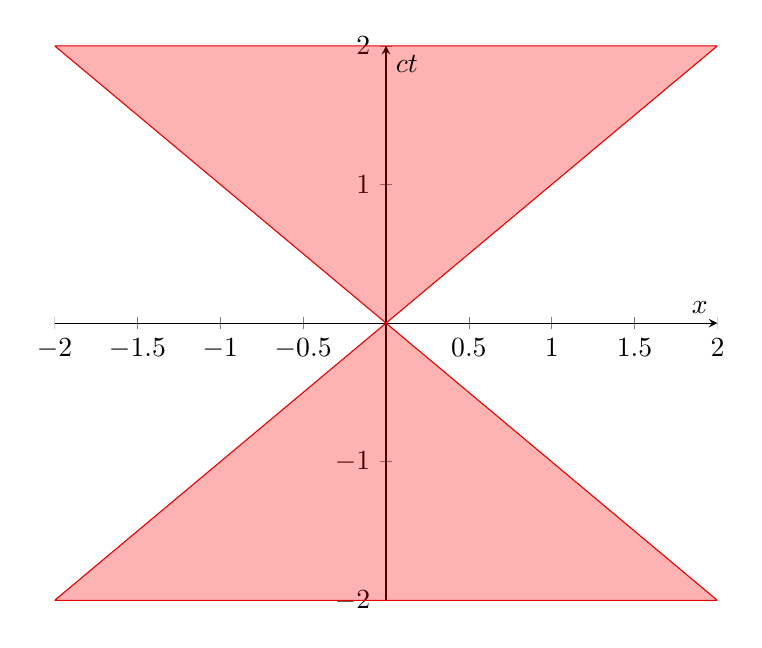
\begin{tikzpicture}
		\begin{axis}[
				axis lines = center,
				xlabel = \(x\),
				ylabel = \(ct\),
			]

			\addplot [red!90!black, fill=red, fill opacity=0.3] coordinates {
					(0, 0) (2, 2) (-2, 2) (2, -2) (-2, -2)
				} -- cycle;
		\end{axis}
	\end{tikzpicture}
\end{center}
We can also draw the axes of a different frame \(S'\) on the same diagram, moving at speed \(v\) relative to \(S\).
The \(t'\) axis corresponds to the equation \(x'=0\) and therefore corresponds to \(x=vt\), or equivalently \(x = \frac{v}{c} \cdot ct\).
The \(x'\) axis corresponds to \(t'=0\), which is \(ct = \frac{v}{c}\cdot x\).
\begin{center}
	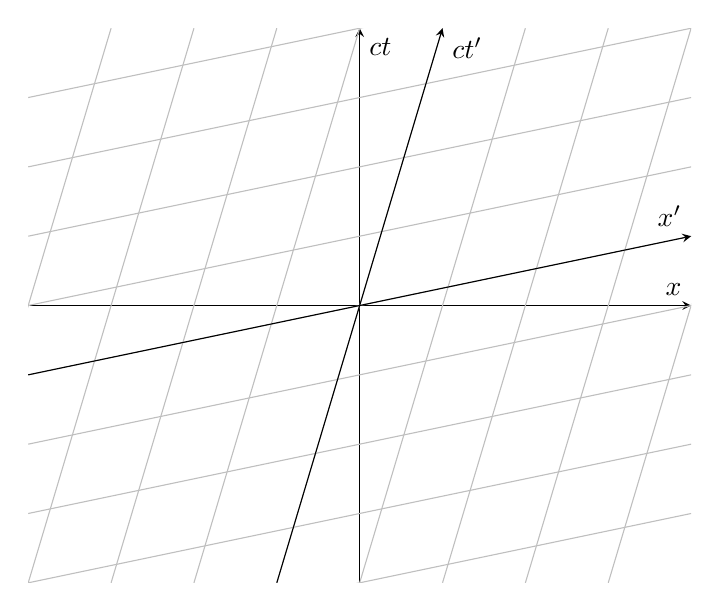
\begin{tikzpicture}
		\begin{axis}[
				axis lines = center,
				xlabel = \(x\),
				ylabel = \(ct\),
				xmin=-2,
				ymin=-2,
				xmax=2,
				ymax=2,
				xtick=\empty,
				ytick=\empty,
			]

			\draw[color=lightgray] (axis cs: -2.5, -2) -- (axis cs: -1.5, 2);
			\draw[color=lightgray] (axis cs: -2, -2) -- (axis cs: -1, 2);
			\draw[color=lightgray] (axis cs: -1.5, -2) -- (axis cs: -0.5, 2);
			\draw[color=lightgray] (axis cs: -1, -2) -- (axis cs: 0, 2);
			\draw[color=lightgray] (axis cs: -0.5, -2) -- (axis cs: 0.5, 2);
			\draw[color=lightgray] (axis cs: 0, -2) -- (axis cs: 1, 2);
			\draw[color=lightgray] (axis cs: 0.5, -2) -- (axis cs: 1.5, 2);
			\draw[color=lightgray] (axis cs: 1, -2) -- (axis cs: 2, 2);
			\draw[color=lightgray] (axis cs: 1.5, -2) -- (axis cs: 2.5, 2);

			\draw[color=lightgray] (axis cs: -2, -2.5) -- (axis cs: 2, -1.5);
			\draw[color=lightgray] (axis cs: -2, -2) -- (axis cs: 2, -1);
			\draw[color=lightgray] (axis cs: -2, -1.5) -- (axis cs: 2, -0.5);
			\draw[color=lightgray] (axis cs: -2, -1) -- (axis cs: 2, 0);
			\draw[color=lightgray] (axis cs: -2, -0.5) -- (axis cs: 2, 0.5);
			\draw[color=lightgray] (axis cs: -2, 0) -- (axis cs: 2, 1);
			\draw[color=lightgray] (axis cs: -2, 0.5) -- (axis cs: 2, 1.5);
			\draw[color=lightgray] (axis cs: -2, 1) -- (axis cs: 2, 2);
			\draw[color=lightgray] (axis cs: -2, 1.5) -- (axis cs: 2, 2.5);

			\draw[->,>=stealth] (axis cs: -0.5, -2) -- (axis cs: 0.5, 2);
			\node[anchor=north west] at (axis cs:0.5,2) {\(ct'\)};
			\draw[->,>=stealth] (axis cs: -2, -0.5) -- (axis cs: 2, 0.5);
			\node[anchor=south east] at (axis cs:2,0.5) {\(x'\)};

		\end{axis}
	\end{tikzpicture}
\end{center}
The angle between the \(x\) and \(x'\) axes matches the angle between the \(ct\) and \(ct'\) axes; they are symmetric about the diagonal (as are the original \(x\) and \(ct\) axes).
Note that the diagonal is given by \(x=ct\) and \(x'=ct'\), which is the same light ray.

\subsection{Comparing velocities}
Consider a particle moving with constant velocity \(u'\) in \(S'\), where \(S'\) is travelling at velocity \(v\) with respect to \(S\).
The world line of the particle in \(S'\) is simply \(x' = u' t'\).
Correspondingly in \(S\), \(x=ut\).
Now, using the Lorentz transformation,
\[
	x=\gamma(x' + vt') = \gamma(u' + v)t'
\]
\[
	t = \gamma\qty(t' + \frac{vx'}{c^2}) = \gamma\qty(1 + \frac{vu'}{c^2})t'
\]
Hence,
\[
	u = \frac{x}{t} = \frac{u' + v}{1 + \frac{u'v}{c^2}}
\]
Note that
\[
	c-u = \frac{(c - u')(c - v)}{1 + \frac{u' v}{c^2}}
\]
which is always positive if \(u'<c\) and \(v<c\).
Therefore, a Lorentz transformation preserves the property that a speed is smaller than the speed of light.

\subsection{Simultaneity}
Two events \(P_1\) and \(P_2\) are simultaneous in \(S\) if they occur at the same time in \(S\).
This is a line parallel to the space axis in the spacetime diagram.
In another reference frame, this line of constant time might be at a different angle.
So events simultaneous in \(S'\) may not correspond to events simultaneous in \(S\).
We can use the above formulae to deduce the exact time that an event happens in a different frame of reference.

\subsection{Causality}
Different observers may disagree on the time ordering of events, but we can construct a viewpoint which gives a consistent description of `cause' and `effect', so special relativity does not break causality.
Note that lines of simultaneity cannot have an angle greater than \(\frac{\pi}{2}\) since the speed of the moving frame must be less than \(c\).
We can construct a `light cone' from all lines or surfaces from an event \(P\) at an angle \(\frac{\pi}{2}\) to the time axis, which represents the possible effects of an event.
\begin{center}
	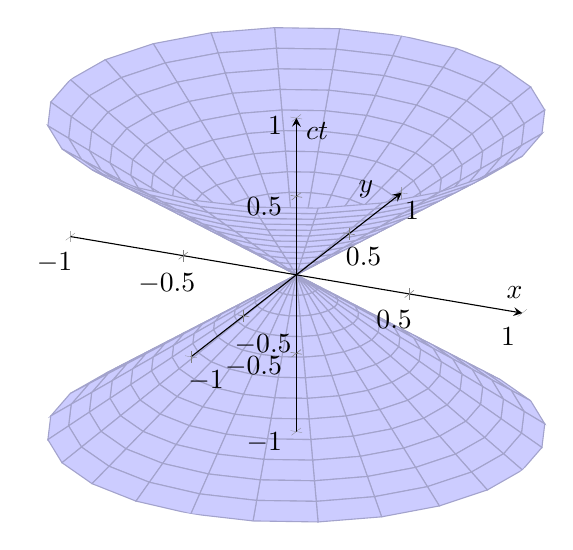
\begin{tikzpicture}
		\begin{axis}[
				axis lines=center,
				axis on top,
				%plot box ratio=1 1 1,
				xlabel=\(x\),
				ylabel=\(y\),
				zlabel={\(ct\)},
				%shader=flat,
				colormap={blue}{rgb=(0.8,0.8,1.0) rgb=(0.8,0.8,1.0)}
			]
			\addplot3 [surf, domain=-1:1, y domain=0:2*pi, z buffer=sort, colormap name=blue] ({x*cos(deg(y))},{x*sin(deg(y))},{x});
		\end{axis}
	\end{tikzpicture}
\end{center}
The cone above the origin is the `future light cone' and the cone below is called the `past light cone'.
Note that this cone is fixed under Lorentz transformations.
If an event occurs in the future light cone, then all observers agree that this event occurs after that the event at the origin.
Likewise, if an event occurs in the past light cone, all observers agree that this event occurs before the event at the origin.
Note that if an event \(P\) is not in the light cone, then it cannot cause, or be caused by, the event at the origin, since nothing travels faster than \(c\).
Hence, an event at the origin can only be influenced by events inside the past light cone, and may only influence events inside the future light cone.

\subsection{Time dilation}
Consider first a clock which is stationary in \(S'\), which ticks at constant intervals \(\Delta t'\).
What is the time interval between ticks as perceived in \(S\)?
We can use the Lorentz transformation, noting that \(x'=0\) since the clock is stationary in \(S'\), to get
\[
	t = \gamma\qty(t' + \frac{vx'}{c^2}) = \gamma t'
\]
Hence,
\[
	\Delta t = \gamma \Delta t'
\]
So moving clocks run slowly.

\subsection{The twin paradox}
Consider two twins \(A\) and \(B\).
Twin \(A\) stays on Earth (considered to be an inertial frame), and \(B\) travels at a constant speed \(v\) to a distant planet \(P\), then she turns around and returns to Earth.
In the frame of reference of \(A\),
\begin{center}
	\begin{tikzpicture}
		\begin{axis}[
				axis lines = left,
				xlabel = \(x\),
				ylabel = \(ct\),
				xtick=\empty,
				ytick=\empty,
				width=4cm,
				height=10cm,
				xmin=0,
				xmax=2.5,
				ymin=0,
				ymax=5,
			]

			%\fill (axis cs:2,1) circle[radius=2pt];
			\node[anchor=south] at (axis cs:1,0) {\(P\)};
			\node[anchor=west] at (axis cs:1,2) {\(E\)};
			\node[anchor=west] at (axis cs:0,4) {\(F\)};
			\draw[dashed,color=lightgray] (axis cs: 1, 0) -- (axis cs: 1, 5);

			\draw[->-=0.5] (axis cs: 0, 0) -- (axis cs: 1, 2);
			\draw[->-=0.5] (axis cs: 1, 2) -- (axis cs: 0, 4);
		\end{axis}
	\end{tikzpicture}
\end{center}
\(E\) is the point where \(B\) reaches \(P\).
The event \(E\) occurs at time \(T\) as perceived by \(A\), so \(E\) has coordinates \((x, ct) = (vT, cT)\).
The time experienced by \(B\) on her outward journey is
\[
	T' = \gamma\qty(T - \frac{v}{c}\cdot vT) = \frac{T}{\gamma}
\]
On her return to event \(F\), twin \(A\) has aged by \(2T\) but twin \(B\) has aged by \(2T' < 2T\).
However, from twin \(B\)'s perspective, twin \(A\) has aged less than she has, since the problem is seemingly symmetric.
This would be a paradox.
To rectify this, consider the frame of reference of \(B\)'s outward journey.
At \(E\), \(x' = 0\) and \(t' = T / \gamma\).
Consider an event \(G\) simultaneous to \(E\) in the frame of reference of \(S'\).
The blue line is a line of constant \(t'\).
\begin{center}
	\begin{tikzpicture}
		\begin{axis}[
				axis lines = left,
				xlabel = \(x\),
				ylabel = \(ct\),
				xtick=\empty,
				ytick=\empty,
				width=4cm,
				height=10cm,
				xmin=0,
				xmax=2.5,
				ymin=0,
				ymax=5,
			]

			%\fill (axis cs:2,1) circle[radius=2pt];
			\node[anchor=south] at (axis cs:1,0) {\(P\)};
			\node[anchor=north west] at (axis cs:1,2) {\(E\)};
			\draw[dashed,color=lightgray] (axis cs: 1, 0) -- (axis cs: 1, 5);
			\draw[color=blue] (axis cs: 0, 1.75) -- (axis cs: 2, 2.25);
			\node[blue,anchor=north west] at (axis cs:0,1.75) {\(G\)};

			\draw[->-=0.5] (axis cs: 0, 0) -- (axis cs: 1, 2);
			\draw[->-=0.5] (axis cs: 1, 2) -- (axis cs: 0, 4);
		\end{axis}
	\end{tikzpicture}
\end{center}
At \(E\),
\[
	t' = \gamma\qty(t - \frac{vx}{c^2}) = t\gamma \implies t = \frac{t'}{\gamma} = \frac{T}{\gamma^2}
\]
So each of them thinks that the other has aged less, when \(B\) is at \(E\), by a factor of \(\gamma^{-1}\).
On the return,
\begin{center}
	\begin{tikzpicture}
		\begin{axis}[
				axis lines = left,
				xlabel = \(x\),
				ylabel = \(ct\),
				xtick=\empty,
				ytick=\empty,
				width=4cm,
				height=10cm,
				xmin=0,
				xmax=2.5,
				ymin=0,
				ymax=5,
			]

			%\fill (axis cs:2,1) circle[radius=2pt];
			\node[anchor=south] at (axis cs:1,0) {\(P\)};
			\node[anchor=west,xshift=0.4cm] at (axis cs:1,2) {\(E\)};
			\draw[dashed,color=lightgray] (axis cs: 1, 0) -- (axis cs: 1, 5);
			\draw[color=red] (axis cs: 0, 2.25) -- (axis cs: 2, 1.75);
			\node[red,anchor=south west] at (axis cs:0,2.25) {\(H\)};
			\draw[color=blue] (axis cs: 0, 1.75) -- (axis cs: 2, 2.25);
			\node[blue,anchor=north west] at (axis cs:0,1.75) {\(G\)};

			\draw[->-=0.5] (axis cs: 0, 0) -- (axis cs: 1, 2);
			\draw[->-=0.5] (axis cs: 1, 2) -- (axis cs: 0, 4);
		\end{axis}
	\end{tikzpicture}
\end{center}
The red line is a line of constant \(t'\) as measured by \(B\) on the return journey, at \(E\).
So for the return journey, \(A\) sees \(B\) age from the event \(E\) to the event \(F\).
However, \(B\) sees \(A\) age from the event \(H\) to the event \(F\).
So there is a time gap between \(G\) and \(H\) as observed by \(B\), which is not considered by the naive model of this problem.
\(B\) sees \(A\) age instantaneously at the point when she changes direction.
In particular, the frame of \(B\) as she changes direction is not inertial.

\subsection{Length contraction}
The length of an object is dependent on the choice of frame.
Consider a rod of length \(L'\) in \(S'\), which is stationary in \(S'\).
The world lines of the ends of the rod are vertical.
The length of the rod at time \(t'\) is the distance in \(x'\) between the two world lines.
In \(S\),
\[
	x' = 0 \implies \gamma(x - vt) = 0
\]
Further,
\[
	x' = L' \implies \gamma(x - vt) = L'
\]
Therefore, the distance between the two \(x\) points at the same \(t\) is \(L = L'/\gamma < L'\).
So the length of a moving object shrinks in the direction it is moving.
Sometimes, analogously to `proper time', we consider the `proper length' of an object, which is the length as measured in the rest frame of the object.

For example, does a train of (proper) length \(2L\) fit alongside a platform of length \(L\) if it is travelling along the tracks at a speed such that \(\gamma = 2\)?
For observers on the platform, the train indeed contracts to length \(L\), so indeed it fits.
On the other hand, for observers on the train, the platform contracts to a length \(\frac{1}{2}L\), so the train would not fit.
To resolve the uncertainty, we will draw a spacetime diagram, from the frame of reference \(S\) where the platform is stationary.
The red lines represent the end points of the platform.
The world lines for the end points of the train are in blue.
\(E\) is the event when the rear of the train is at the rear of the platform, and \(F\) is the event where the front of the train is at the front of the platform.
\begin{center}
	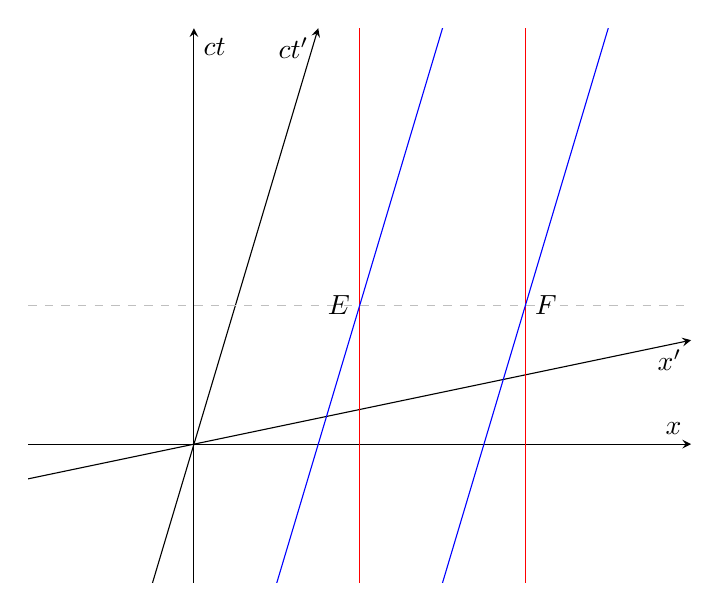
\begin{tikzpicture}
		\begin{axis}[
				axis lines = center,
				xlabel = \(x\),
				ylabel = \(ct\),
				xtick=\empty,
				ytick=\empty,
				xmin=-1,
				xmax=3,
				ymin=-1,
				ymax=3,
			]

			\draw[->,>=stealth] (axis cs: -0.5, -2) -- (axis cs: 0.75, 3);
			\node[anchor=north east] at (axis cs:0.75,3) {\(ct'\)};
			\draw[->,>=stealth] (axis cs: -2, -0.5) -- (axis cs: 3, 0.75);
			\node[anchor=north east] at (axis cs:3,0.75) {\(x'\)};

			\draw[color=red] (axis cs: 1, -1) -- (axis cs: 1, 3);
			\draw[color=red] (axis cs: 2, -1) -- (axis cs: 2, 3);

			\draw[dashed,color=lightgray] (axis cs: -1, 1) -- (axis cs: 3, 1);
			\node[anchor=east] at (axis cs:1, 1) {\(E\)};
			\node[anchor=west] at (axis cs:2, 1) {\(F\)};

			\draw[color=blue] (axis cs: 0, -3) -- (axis cs: 2, 5);
			\draw[color=blue] (axis cs: 1, -3) -- (axis cs: 3, 5);

			%\draw[dashed,color=lightgray] (axis cs: 1, 0) -- (axis cs: 2, 5);
		\end{axis}
	\end{tikzpicture}
\end{center}
Let \(E\) correspond to \(t = 0\) and \(t' = 0\).
The front of the train is at \(x' = 2L\), and the front of the platform is at \(x = L\).
In the \(S\) frame, events \(E\) and \(F\) occur at the same time \(t = 0\).
\[
	x' = \gamma(x - vt) \implies 2L = \gamma(L - vt) = 2(L - vt) \implies t = 0
\]
Further,
\[
	x = \gamma(x' + vt') \implies L = \gamma(2L + vt') = 2(2L + vt') \implies t' = \frac{L - 4 L}{2v} = \frac{-3L}{2v} < 0
\]
Hence, the time \(t'\) at which \(F\) occurs is before the event \(E\).
So from the perspective of the train, the front of the train has already passed the front of the platform by the time that the back of the train passes the back of the platform, so from this perspective the train does not fit.

\section{Geometry of spacetime}
\subsection{Invariant interval}
Consider two events \(P\) and \(Q\) with space-time coordinates \((ct_1, x_1)\) and \((ct_2, x_2)\), where the time coordinate is given first.
The time separation is \(\Delta t = t_1 - t_2\), and the space separation \(\Delta x = x_1 - x_2\).
These two separations are dependent on the choice of inertial frame.
The invariant interval between \(P\) and \(Q\) is defined as
\[
	\Delta s^2 = c^2 \Delta t^2 - \Delta x^2
\]
This is invariant under a Lorentz transformation.
%TODO show this
In three spatial dimensions, we simply replace this \(\Delta x^2\) with \(\Delta x^2 + \Delta y^2 + \Delta z^2\), so
\[
	\Delta s^2 = c^2 \Delta t^2 - \Delta x^2 - \Delta y^2 - \Delta z^2
\]
If the separation between \(P\) and \(Q\) is very small, we can define the infinitesimal invariant interval as
\[
	\dd{s}^2 = c^2\dd{t}^2 - \dd{x}^2 - \dd{y}^2 - \dd{z}^2
\]
Note that spacetime with three spatial dimensions (Minkowski spacetime) is topologically equivalent to \(\mathbb R^4\), where the distance measure is \(\dd{s}^2\) as defined above.
Note that this distance quantity, although squared, can be either positive or negative.
Sometimes this arrangement of one temporal and three spatial dimensions is denoted by the abbreviation `\(1+3\) dimensions'.

\subsection{Signs of the invariant interval}
As noted before, \(\Delta s^2\) can have either a positive or negative sign.
\begin{itemize}
	\item Events with \(\Delta s^2 > 0\) are `time-like separated'.
	      In this case, there exists a frame of reference in which the events occur in the same spatial position, but at different times.
	      In particular, the two events appear in each other's light cones.
	      The time ordering of the two events is unambiguous.
	\item Events with \(\Delta s^2 < 0\) are `space-like separated'.
	      Here, there exists a frame of reference in which the events occur at the same time, but in different places.
	      The two events are outside of each other's light cones, and the ordering of the two events can change depending on the choice of frame of reference.
	\item If \(\Delta s^2 = 0\), the events are `light-like separated'.
	      The events lie exactly on each other's light cones, and this does \textit{not} imply that the two events are the same (unlike in Euclidean space, where a distance measure of zero implies that two points are equal).
\end{itemize}

\subsection{The Lorentz group}
The coordinates of an event \(P\) in some frame \(S\) can be written as a 4-vector \(X\).
\[
	X^\mu = \begin{pmatrix}
		ct \\ x \\ y \\ z
	\end{pmatrix}
\]
where the \(ct\) coordinate is given by \(\mu = 0\) and the spatial dimensions are given by \(\mu = 1, 2, 3\) as usual.
The invariant interval betwen \(P\) and the origin is written as the inner product of \(X\) with itself:
\[
	X \cdot X \coloneq X^\transpose \eta X
\]
or alternatively,
\[
	X \cdot X = \eta_{\mu\nu} X^\mu X^\nu
\]
where \(\eta\) is the Minkowski metric given by
\[
	\eta = \begin{pmatrix}
		1 & 0  & 0  & 0  \\
		0 & -1 & 0  & 0  \\
		0 & 0  & -1 & 0  \\
		0 & 0  & 0  & -1
	\end{pmatrix}
\]
Then
\[
	X \cdot X = c^2t^2 - x^2 - y^2 - z^2
\]
We can classify 4-vectors as `space-like', `time-like' and `light-like' as before, by considering the sign of \(\eta_{\mu\nu}X^\mu X^\nu\).
The Lorentz transformation is a linear transformation that converts the components of \(X\) into the components of \(X\) in \(S'\).
Therefore, any Lorentz transform can be represented as a \(4\times 4\) matrix \(\Lambda\).
We now define Lorentz transforms as such linear transformations that preserve the Minkowski metric.
So considering a sets of coordinates \(X\) and \(X'\) in \(S\) and \(S'\), we have \(X' = \Lambda X\), and \(X' \cdot X' = X \cdot X\).
This then implies that
\begin{equation}
	\Lambda^\transpose \eta \Lambda = \eta \tag{\(\ast\)}
\end{equation}
Two classes of possible \(\Lambda\) are
\[
	\Lambda = \begin{pmatrix}
		1 & 0 & 0 & 0 \\
		0 & a & b & c \\
		0 & d & e & f \\
		0 & g & h & i
	\end{pmatrix};\quad R = \begin{pmatrix}
		a & b & c \\
		d & e & f \\
		g & h & i
	\end{pmatrix}
\]
where \(R^\transpose R = I\), giving that \(R\) may be a spatial rotation or a reflection.
We could also have
\[
	\Lambda = \begin{pmatrix}
		\gamma       & -\gamma\beta & 0 & 0 \\
		-\gamma\beta & \gamma       & 0 & 0 \\
		0            & 0            & 1 & 0 \\
		0            & 0            & 0 & 1
	\end{pmatrix}
\]
where \(\beta = \frac{v}{c}\).
This expresses a Lorentz transformation where the two frames are moving at a constant velocity \(v\) relative to each other, as discussed before in \(1+1\) spacetime.
We denote the Lorentz group as \(O(1, 3)\), defined by the set of \(\Lambda\) that satisfy \((\ast)\).
Note that this includes the group generated by the above two transformations (notably including spatial reflections), as well as time reflections.
We define the \textit{proper} Lorentz group as \(SO(1, 3)\), which is the kernel of the determinant homomorphism on the Lorentz group.
Note that this includes the \textit{composition} of both temporal and spatial reflection.
The subgroup that forbids any kind of reflection is called the \textit{restricted} Lorentz group, denoted \(SO^+(1, 3)\), generated by compositions of rotations and boosts, as shown in the above two examples (excluding the case when \(R\) is a reflection).

\subsection{Rapidity}
While a \(4\times 4\) matrix can be useful for computation, it is sometimes more convenient to label a Lorentz transformation using a concept of `rapidity'.
In \(1+1\) spacetime, we write
\[
	\Lambda[\beta] = \begin{pmatrix}
		\gamma       & -\gamma\beta \\
		-\gamma\beta & \gamma
	\end{pmatrix};\quad \gamma = (1 - \beta^2)^{-\frac{1}{2}}
\]
This represents a boost in the \(x\) direction.
Combining two boosts, we get
\begin{align*}
	\Lambda[\beta_1]\Lambda[\beta_2] &= \begin{pmatrix}
		\gamma_1         & -\gamma_1\beta_1 \\
		-\gamma_1\beta_1 & \gamma_1
	\end{pmatrix}\begin{pmatrix}
		\gamma_2         & -\gamma_2\beta_2 \\
		-\gamma_2\beta_2 & \gamma_2
	\end{pmatrix} \\
	&= \begin{pmatrix}
		\gamma_1\gamma_2(1 + \beta_1 \beta_2) & -\gamma_1\gamma_2(\beta_1 + \beta_2)  \\
		-\gamma_1\gamma_2(\beta_1 + \beta_2)  & \gamma_1\gamma_2(1 + \beta_1 \beta_2)
	\end{pmatrix} \\
	&= \Lambda\qty[\frac{\beta_1 + \beta_2}{1 + \beta_1\beta_2}]
\end{align*}
Note the relation to the velocity transformation law.
Recall that with spatial rotations, we can characterise a rotation \(R\) by some parameter \(\theta\), where \(R(\theta_1) R(\theta_2) = R(\theta_1 + \theta_2)\).
This is the same kind of composition law.
For Lorentz boosts, we can define \(\phi\) such that \(\beta = \tanh\phi\), and then we can redefine \(\Lambda\) to be in terms of \(\phi\), giving this new composition law
\[
	\Lambda[\phi_1]\Lambda[\phi_2] = \Lambda[\phi_1 + \phi_2]
\]
Note that \(\gamma = \cosh \phi\), and \(\gamma\beta = \sinh \phi\).
This suggests that Lorentz boosts can be thought of as hyperbolic rotations in spacetime.

\section{Relativistic physics}
\subsection{Proper time}
A particle moves along a trajectory \(\vb x(t)\).
The velocity of this particle is \(\dv{\vb x}{t} = \vb u(t)\).
The path in spacetime is parametrised by \(t\).
Both \(\vb x\) and \(t\) vary under a Lorentz transformation.
Now, consider a particle at rest in \(S'\) with \(\vb x' = 0\).
The invariant interval on the world line is
\[
	\Delta s^2 = c^2 \Delta t^2
\]
We define the proper time \(\tau\) as
\[
	\Delta \tau = \frac{1}{c}\Delta s
\]
In particular, in \(S'\), \(\Delta\tau = \Delta t\), so the proper time is the time experienced in the rest frame of the particle.
However, the equation \(\Delta \tau = \frac{1}{c}\Delta s\) holds in all frames, since \(\Delta s\) is Lorentz invariant.
Note further that \(\Delta s\) is real since this always represents a timelike interval, as it represents a particle travelling through spacetime.
We can therefore instead parametrise this particle's world line by its proper time, rather than by considering the time in any particular frame.
So \(\vb x\) and \(t\) are both functions of \(\tau\) in any given reference frame.
Further, infinitesimal changes are related by
\begin{align*}
	\dd{\tau}               & = \frac{\dd{s}}{c}                                       \\
	                        & = \frac{1}{c}\sqrt{c^2\dd{t}^2 - \abs{\dd{\vb x}}^2}     \\
	                        & = \frac{1}{c}\sqrt{c^2\dd{t}^2 - \abs{\vb u}^2 \dd{t}^2} \\
	                        & = \qty(1 - \frac{\vb u^2}{c^2})^{\frac{1}{2}}\dd{t}      \\
	\therefore\ \dv{t}{\tau} & = \gamma_{\vb u}
\end{align*}
where \(\gamma_{\vb u} = \qty(1 - \frac{\vb u^2}{c^2})^{\frac{1}{2}}\).
Now, the total time observed by a particle moving along its world line is
\[
	T = \int \dd{\tau} = \int \frac{\dd{t}}{\gamma_{\vb u}}
\]

\subsection{4-velocity}
We can parametrise the position 4-vector of a particle using \(\tau\), written
\[
	X(\tau) = \begin{pmatrix}
		ct(\tau) \\ \vb x(\tau)
	\end{pmatrix}
\]
We define the 4-velocity as
\[
	U = \dv{\tau}X = \begin{pmatrix}
		c\dv*{t}{\tau} \\ \dv*{\vb x}{\tau}
	\end{pmatrix} = \dv{t}{\tau} \begin{pmatrix}
		c \\ \vb u
	\end{pmatrix} = \gamma_{\vb u} \begin{pmatrix}
		c \\ \vb u
	\end{pmatrix}
\]
Since \(X' = \Lambda X\), we also have that
\[
	U' = \Lambda U
\]
because \(\tau\) is invariant.
Note that any quantity whose components transform according to this rule is called a 4-vector, and in particular, the derivative of a 4-vector with respect to an invariant is also a 4-vector.
Also, the scalar product \(U \cdot U\) is invariant under Lorentz transforms.
Indeed, in the rest frame of a particle moving with 4-velocity \(U\), in this frame we have \(U\cdot U = c^2\).
In other frames,
\[
	U \cdot U = \gamma^2 (c^2 - \vb u^2) = c^2
\]
as expected.

\subsection{Transformation of velocities}
We have found that in special relativity, we cannot simply add velocities together.
Consider a transformation \(\Lambda\) from \(S\) to \(S'\), where \(S'\) is moving (relative to \(S\)) at a speed \(v\) in the \(x\) direction.
Consider a particle moving in \(S\) at speed \(u\) at an angle \(\theta\) to the \(x\) axis (with no component in the \(z\) axis).
In \(S'\), it moves with speed \(u'\) at an angle \(\theta'\).
We can write the 4-velocities as
\[
	U = \begin{pmatrix}
		\gamma_{\vb u}c           \\
		\gamma_{\vb u}u\cos\theta \\
		\gamma_{\vb u}u\sin\theta \\
		0
	\end{pmatrix};\quad U' = \begin{pmatrix}
		\gamma_{\vb u'}c             \\
		\gamma_{\vb u'}u'\cos\theta' \\
		\gamma_{\vb u'}u'\sin\theta' \\
		0
	\end{pmatrix}
\]
and further,
\[
	U' = \Lambda U
\]
where
\[
	\Lambda = \begin{pmatrix}
		\gamma_v              & -\gamma_v \frac{v}{c} & 0 & 0 \\
		-\gamma_v \frac{v}{c} & \gamma_v              & 0 & 0 \\
		0                     & 0                     & 1 & 0 \\
		0                     & 0                     & 0 & 1
	\end{pmatrix}
\]
Carrying out the matrix multiplication, we find
\[
	\begin{pmatrix}
		\gamma_{\vb u'}c             \\
		\gamma_{\vb u'}u'\cos\theta' \\
		\gamma_{\vb u'}u'\sin\theta' \\
		0
	\end{pmatrix} = \begin{pmatrix}
		\gamma_v              & -\gamma_v \frac{v}{c} & 0 & 0 \\
		-\gamma_v \frac{v}{c} & \gamma_v              & 0 & 0 \\
		0                     & 0                     & 1 & 0 \\
		0                     & 0                     & 0 & 1
	\end{pmatrix} \begin{pmatrix}
		\gamma_{\vb u}c           \\
		\gamma_{\vb u}u\cos\theta \\
		\gamma_{\vb u}u\sin\theta \\
		0
	\end{pmatrix} \implies \left\{ \begin{array}{l}
		\displaystyle
		u'\cos\theta' = \frac{u\cos\theta - v}{1 - uv\cos\theta/c^2}      \\
		\displaystyle
		\tan\theta' = \frac{u\sin\theta}{\gamma_{\vb u}(u\cos\theta - v)} \\
	\end{array} \right.
\]
The first equation corresponds to the normal transformation law for Lorentz transforms.
The second equation, corresponding to a change in angle due to the motion of the observer, is called aberration.
In particular, when \(u = c\), we can see that light rays appear to change direction due to the relative motion of the emitter and the observer.

\subsection{Energy-momentum 4-vector}
We define the 4-momentum of a particle of mass \(m\) and 4-velocity \(U\) to be
\[
	P = mU = m\gamma_{\vb u} \begin{pmatrix}
		c \\ \vb u
	\end{pmatrix}
\]
Since \(U\) is a 4-vector, we must have that \(m\) is invariant under a Lorentz transformation.
We will call this \(m\) the `rest mass' of the object, defined as the mass as measured in the rest frame of the particle.
The 4-momentum of a system of particles is defined as the sum of the 4-momenta of its individual particles.
The spatial components of \(P\), given by \(\mu = 1, 2, 3\), can be referred to as the relativistic 3-momentum, given by \(\vb p = \gamma_{\vb u} m \vb u\).
This matches with the definition as seen in Newtonian physics, except that the mass \(m\) is replaced by \(\gamma_{\vb u} m\).
We call this quantity the `apparent mass' of the particle or system of particles, as it represents the mass of the particle as observed by a different reference frame.
Note that \(\abs{\vb p}\) and \(\gamma_{\vb u} m\) both tend to infinity as the particle approaches the speed of light.
Note that the first component of \(P\), \(P^0\), is
\[
	\gamma_{\vb u} mc = \frac{mc}{\sqrt{1 - \frac{\vb u^2}{c^2}}} = \frac{1}{c}\qty(mc^2 + \frac{1}{2}m\vb u^2 + \dots)
\]
We recognise the \(\frac{1}{2}m\vb u^2\) term as the kinetic energy of the particle.
We interpret \(P^0\) as an energy, divided by \(c\) (to conserve units).
\[
	P = \begin{pmatrix}
		\frac{1}{c} E \\ \vb p
	\end{pmatrix}
\]
where
\[
	E = \gamma_{\vb u} mc^2 = mc^2 + \frac{1}{2}m\vb u^2 + \dots
\]
Note that as \(\abs{\vb u} \to c\), \(E \to \infty\).
Since \(P\) contains an energy term as well as a momentum term, we also call \(P\) the energy-momentum 4-vector.
Note that for a stationary particle of rest mass \(m\), we have
\[
	E = mc^2
\]
This implies that mass is a form of energy.
The energy of a moving particle is
\[
	E = mc^2 + \underbrace{(\gamma_{\vb u} - 1)mc^2}_{\mathclap{\text{relativistic kinetic energy}}}
\]
Since \(P \cdot P = \frac{E^2}{c^2} - \abs{\vb p}^2\) is Lorentz invariant, we have
\[
	P \cdot P = m^2c^2
\]
Hence,
\[
	\frac{E^2}{c^2} = \abs{\vb p}^2 + m^2c^2
\]
In Newtonian physics, mass is conserved, and energy is also conserved.
In relativistic physics, mass is not conserved by itself, since it is a form of energy.
From this derivation, it is theoretically possible to convert between mass and kinetic energy.

\subsection{Massless particles}
A massless particle has zero rest mass.
Such particles can have nonzero momentum and nonzero energy, because they are travelling at the speed of light, giving \(\gamma_{\vb u} = \infty\).
Since \(P \cdot P = m^2c^2\), there are no factors of \(\gamma\) in this expression giving
\[
	P \cdot P = 0
\]
So such a particle travels along a light-like trajectory.
Therefore there is no Lorentz transformation that brings a given reference frame into the rest frame of the particle, so we cannot define proper time for such a particle.
Since \(m^2c^2 = 0\), we must have
\[
	\frac{E^2}{c^2} = \abs{\vb p}^2 \implies E = \abs{\vb p}c
\]
Then,
\[
	P = \frac{E}{c} \begin{pmatrix}
		1 \\ \vu n
	\end{pmatrix}
\]
where \(\vu n\) is a unit 3-vector in the direction of travel of the particle.

\subsection{Newton's second law}
Now that we have defined \(P\) for all particles, we can rewrite Newton's second law in special relativity as
\[
	\dv{P}{\tau} = F
\]
where \(F\) is the 4-force.
If the 3-force is \(\vb F\), we have
\[
	F = \gamma_{\vb u} \begin{pmatrix}
		\vb F \cdot \vb u / c \\
		\vb F
	\end{pmatrix}
\]
Hence,
\[
	\dv{E}{\tau} = \gamma_{\vb u} \vb F \cdot \vb u;\quad \dv{\vb p}{\tau} = \gamma_{\vb u} \vb F
\]
giving
\[
	\dv{E}{t} = \vb F \cdot \vb u;\quad \dv{\vb p}{t} = \vb F
\]
which are the familiar Newtonian expressions for rate of work and rate of change of momentum.
We can now define 4-acceleration:
\[
	F = mA
\]
where \(m\) is the rest mass.
Hence,
\[
	\dv{U}{\tau} = A
\]

\subsection{Special relativity with particle physics}
In Newtonian physics, when two particles collide, we must consider the conservation of 3-momentum.
In special relativity however, we must instead consider the conservation of 4-momentum:
\[
	P = \begin{pmatrix}
		\frac{E}{c} \\ \vb p
	\end{pmatrix}
\]
It is often convenient, when dealing with systems of particles, to let the origin of our frame of reference be the centre of momentum.
This is the frame such that the total 3-momentum of the system is zero.
However, this cannot be done when dealing with massless particles since there does not exist such a rest frame.

\subsection{Particle decay}
Consider a particle of mass \(m_1\) with 3-momentum \(\vb p_1\) which decays into two particles of mass \(m_2\) and \(m_3\) with 3-momenta \(\vb p_2, \vb p_3\).
Since 4-momentum is conserved, we get \(P_1 = P_2 + P_3\).
First, consider the 0 component (the timelike component) of \(P\).
\[
	E_1 = E_2 + E_3
\]
Now, consider the \(1, 2, 3\) components (the spacelike components) of the 4-momentum.
We have
\[
	\vb p_1 = \vb p_2 + \vb p_3
\]
Let us look at this in the centre of momentum frame, so \(\vb p_1 = 0\).
Hence
\[
	\vb p_2 = -\vb p_3
\]
Because we are in the centre of momentum frame, we have \(E_1 = m_1 c^2\) hence
\[
	\frac{E_1}{c} = m_1 c = \frac{E_2}{c} + \frac{E_3}{c}
\]
Further,
\[
	\frac{E_2}{c} = \sqrt{\vb p_2^2 + m_2^2 c^2};\quad \frac{E_3}{c} = \sqrt{\vb p_3^2 + m_3^2 c^2}
\]
Hence,
\[
	m_1 c = \sqrt{\vb p_2^2 + m_2^2 c^2} + \sqrt{\vb p_3^2 + m_3^2 c^2} \geq m_2 c + m_3 c
\]
Hence the rest mass of the initial particle must be \textit{at least} the sum of the rest masses of the particles that result from the decay.

\subsection{Higgs to photon decay}
Consider the decay of the Higgs particle \(h\) into two photons \(\gamma_1, \gamma_2\).
By conservation of 4-momentum,
\[
	P_h = P_{\gamma_1} + P_{\gamma_2}
\]
In the Higgs rest frame,
\[
	P_h = \begin{pmatrix}
		m_h c \\ \vb 0
	\end{pmatrix} =
	\begin{pmatrix}
		\frac{E_{\gamma_1}}{c} \\ \vb p_{\gamma_1}
	\end{pmatrix}
	+
	\begin{pmatrix}
		\frac{E_{\gamma_2}}{c} \\ \vb p_{\gamma_2}
	\end{pmatrix}
\]
Looking at the \(1, 2, 3\) components we find
\[
	\vb p_{\gamma_1} = -\vb p_{\gamma_2}
\]
Looking at the 0 component we find
\[
	m_h c = \frac{E_{\gamma_1}}{c} + \frac{E_{\gamma_2}}{c}
\]
Since \(\frac{E^2}{c^2} = \vb p^2 + m^2c^2\), because the photons have zero rest mass we have
\[
	\frac{E_{\gamma_1}}{c} = \abs{\vb p_{\gamma_1}} = \abs{\vb p_{\gamma_2}} = \frac{E_{\gamma_2}}{c}
\]
Hence,
\[
	E_{\gamma_1} = E_{\gamma_2} = \frac{1}{2}m_h c^2
\]
Note that mass has been lost, but kinetic energy has been gained.

\subsection{Particle scattering}
Consider two identical particles colliding, without decaying into new particles.
In frame \(S\), particle 1 is moving horizontally with 3-velocity \(\vb u\), and particle 2 starts at rest.
After the collision, particle 1 has 3-velocity \(\vb q\) and particle 2 has 3-velocity \(\vb r\), where \(\vb q\) has angle \(\theta\) to the horizontal and \(\vb r\) has angle \(\phi\) to the horizontal.
In the centre of momentum frame \(S'\), particles 1 and 2 move towards each other horizontally with 3-momenta \(\vb p_1\) and \(\vb p_2 = -\vb p_1\).
After the collision, particle 1 moves with 3-momentum \(\vb p_3\) and particle 2 moves with 3-momentum \(\vb p_4 = -\vb p_3\).
The angle of deflection is \(\theta'\).
By conservation of 4-momentum,
\[
	P_1 + P_2 = P_3 + P_4
\]
Since particles 1 and 2 have the same mass, their speeds (in \(S'\)) are equal both before and after the collision.
Let the speed before the collision be \(v\) and the speed after the collision be \(w\).
\[
	P_1' = \begin{pmatrix}
		m\gamma_v c \\
		m\gamma_v v \\
		0           \\
		0
	\end{pmatrix};\quad P_2' = \begin{pmatrix}
		m\gamma_v c  \\
		-m\gamma_v v \\
		0            \\
		0
	\end{pmatrix};\quad P_3' = \begin{pmatrix}
		m\gamma_w c             \\
		m\gamma_w w \cos\theta' \\
		m\gamma_w w \sin\theta' \\
		0
	\end{pmatrix};\quad P_4' = \begin{pmatrix}
		m\gamma_w c              \\
		-m\gamma_w w \cos\theta' \\
		-m\gamma_w w \sin\theta' \\
		0
	\end{pmatrix}
\]
Looking at the 0 component,
\[
	2 m\gamma_v c = 2m\gamma_w c
\]
Since \(m\) is the same on both sides,
\[
	v = w
\]
Now we will apply a Lorentz transformation to return to \(S\).
\[
	\Lambda = \begin{pmatrix}
		\gamma_v             & \gamma_v \frac{v}{c} & 0 & 0 \\
		\gamma_v \frac{v}{c} & \gamma_v             & 0 & 0 \\
		0                    & 0                    & 1 & 0 \\
		0                    & 0                    & 0 & 1
	\end{pmatrix}
\]
Now, since \(u\) is the initial velocity of particle 1 in \(S\),
\[
	P_1 = \Lambda P_1' = \begin{pmatrix}
		m\gamma_v^2 \qty(c + \frac{v^2}{c}) \\
		m\gamma_v^2 (v+v)                   \\
		0                                   \\
		0
	\end{pmatrix} = \begin{pmatrix}
		m\gamma_u c \\
		m\gamma_u u \\
		0           \\
		0
	\end{pmatrix}
\]
After the collision, as seen in \(S\), particle 1's 4-momentum is
\[
	P_3 = \Lambda P_3' = \begin{pmatrix}
		m\gamma_v^2 \qty(c + \frac{v^2}{c}\cos\theta') \\
		m\gamma_v^2 \qty(v + v\cos\theta')             \\
		m\gamma_v v\sin\theta'                         \\
		0
	\end{pmatrix} = \begin{pmatrix}
		m\gamma_q c           \\
		m\gamma_q q\cos\theta \\
		m\gamma_q q\sin\theta \\
		0
	\end{pmatrix}
\]
By dividing the 1 and 2 components on both sides, we deduce
\[
	\tan\theta = \frac{m\gamma_v v\sin\theta'}{m\gamma_v^2 v(1 + \cos\theta')} = \frac{1}{\gamma_v} \tan\frac{1}{2}\theta'
\]
For the second particle, we can do the same calculation to get
\[
	\tan\phi = \frac{m\gamma_v v\sin\theta'}{m\gamma_v^2 v(1 - \cos\theta')} = \frac{1}{\gamma_v} \cot\frac{1}{2}\theta'
\]
So given the knowledge of the exact setup of the particles, we can find the angles between the particles as viewed in a different reference frame.
In particular,
\[
	\tan\theta \cdot \tan\phi = \frac{1}{\gamma_v^2} = \frac{2}{1+\gamma_u} \leq 1
\]
This is a generalisation of the Newtonian result, where \(\gamma_u = 1\) giving
\[
	\tan\theta \cdot \tan\phi = 1
\]
So the angle between the trajectories in the Newtonian case is \(\frac{\pi}{2}\).

\subsection{Particle creation}
Consider equal particles 1 and 2 of mass \(m\) moving towards each other horizontally with speed \(v\) in \(S\), with 4-momenta \(P_1\) and \(P_2\).
After the collision, particles 1 and 2 have 4-momenta \(P_3\) and \(P_4\), and a new particle 3 with 4-momentum \(P_5\) is created with mass \(M\).
Note that \(S\) is the centre of momentum frame.
By conservation of 4-momentum, we have
\[
	P_1 + P_2 = P_3 + P_4 + P_5
\]
We have
\[
	P_2 + P_2 = \begin{pmatrix}
		2m\gamma_v c \\ \vb 0
	\end{pmatrix} = \begin{pmatrix}
		\frac{E_3}{c} + \frac{E_4}{c} + \frac{E_5}{c} \\
		\vb 0
	\end{pmatrix}
\]
Certainly we have
\[
	2m\gamma_v c^2 = E_3 + E_4 + E_5 \geq (m + m + M)c^2 = (2m + M)c^2
\]
Hence, for the particle's creation to be possible, we must have
\[
	\gamma_v \geq 1 + \frac{M}{2m}
\]
So the initial kinetic energy in \(S\) must satisfy
\[
	2m(\gamma_v - 1)c^2 \geq Mc^2
\]
Consider some other reference frame \(S'\) where one particle moves with speed \(u\) and the other is at rest.
Then
\[
	u = \frac{2v}{1 + \frac{v^2}{c^2}}
\]
Hence, by the result above in the particle scattering experiment,
\[
	\gamma_u = 2(\gamma_v^2 - 1) \geq 2\qty(1 + \frac{M}{2m})^2 - 1 = 1 + \frac{2M}{m} + \frac{M^2}{2m^2}
\]
Hence, in this frame, the kinetic energy \(mc^2(\gamma_u - 1)\) must satisfy
\[
	mc^2(\gamma_u - 1) \geq mc^2\qty(\frac{2M}{m} + \frac{M^2}{2m^2}) \geq 2Mc^2 + \frac{M^2c^2}{2m}
\]
This extra \(\frac{M^2c^2}{2m}\) term (compared to the \(Mc^2\) expression in \(S\)) is produced by the transformation between frames.
So in a frame where one particle is at rest, we require significantly more kinetic energy.
So a particle accelerator is most efficiently utilised by accelerating two particles into each other, rather than by accelerating one particle into a fixed target.


\end{document}
